%%%%%%%%%%%%%%%%%%%%%%%%%%%%%%%%%%%%%%%%%%%%%%%%%%%%%%%%%%%%%%%%%%%%%%%%%%%%%%%%
%%%%%%%%%%%%%%%%%%%%%%%%%%%%%%%%%%%%%%%%%%%%%%%%%%%%%%%%%%%%%%%%%%%%%%%%%%%%%%%%
%%                                                                            %%
%% thesistemplate.tex version 3.20 (2018/08/31)                               %%
%% The LaTeX template file to be used with the aaltothesis.sty (version 3.20) %%
%% style file.                                                                %%
%% This package requires pdfx.sty v. 1.5.84 (2017/05/18) or newer.            %%
%%                                                                            %%
%% This is licensed under the terms of the MIT license below.                 %%
%%                                                                            %%
%% Written by Luis R.J. Costa.                                                %%
%% Currently developed at the Learning Services of Aalto University School of %%
%% Electrical Engineering by Luis R.J. Costa since May 2017.                  %%
%%                                                                            %%
%% Copyright 2017-2018, by Luis R.J. Costa, luis.costa@aalto.fi,              %%
%% Copyright 2017-2018 Swedish translations in aaltothesis.cls by Elisabeth   %%
%% Nyberg, elisabeth.nyberg@aalto.fi and Henrik Wallén,                       %%
%% henrik.wallen@aalto.fi.                                                    %%
%% Copyright 2017-2018 Finnish documentation in the template opinnatepohja.tex%%
%% by Perttu Puska, perttu.puska@aalto.fi, and Luis R.J. Costa.               %%
%% Copyright 2018 English template thesistemplate.tex by Luis R.J. Costa.     %%
%% Copyright 2018 Swedish template kandidatarbetsbotten.tex by Henrik Wallen. %%
%%                                                                            %%
%% Permission is hereby granted, free of charge, to any person obtaining a    %%
%% copy of this software and associated documentation files (the "Software"), %%
%% to deal in the Software without restriction, including without limitation  %%
%% the rights to use, copy, modify, merge, publish, distribute, sublicense,   %%
%% and/or sell copies of the Software, and to permit persons to whom the      %%
%% Software is furnished to do so, subject to the following conditions:       %%
%% The above copyright notice and this permission notice shall be included in %%
%% all copies or substantial portions of the Software.                        %%
%% THE SOFTWARE IS PROVIDED "AS IS", WITHOUT WARRANTY OF ANY KIND, EXPRESS OR %%
%% IMPLIED, INCLUDING BUT NOT LIMITED TO THE WARRANTIES OF MERCHANTABILITY,   %%
%% FITNESS FOR A PARTICULAR PURPOSE AND NONINFRINGEMENT. IN NO EVENT SHALL    %%
%% THE AUTHORS OR COPYRIGHT HOLDERS BE LIABLE FOR ANY CLAIM, DAMAGES OR OTHER %%
%% LIABILITY, WHETHER IN AN ACTION OF CONTRACT, TORT OR OTHERWISE, ARISING    %%
%% FROM, OUT OF OR IN CONNECTION WITH THE SOFTWARE OR THE USE OR OTHER        %%
%% DEALINGS IN THE SOFTWARE.                                                  %%
%%                                                                            %%
%%                                                                            %%
%%%%%%%%%%%%%%%%%%%%%%%%%%%%%%%%%%%%%%%%%%%%%%%%%%%%%%%%%%%%%%%%%%%%%%%%%%%%%%%%
%%                                                                            %%
%%                                                                            %%
%% An example for writting your thesis using LaTeX                            %%
%% Original version and development work by Luis Costa, changes to the text   %%
%% in the Finnish template by Perttu Puska.                                   %%
%% Support for Swedish added 15092014                                         %%
%% PDF/A-b support added on 15092017                                          %%
%% PDF/A-2 support added on 24042018                                          %%
%%                                                                            %%
%% This example consists of the files                                         %%
%%         thesistemplate.tex (version 3.20) (for text in English)            %%
%%         opinnaytepohja.tex (version 3.20) (for text in Finnish)            %%
%%         kandidatarbetsbotten.tex (version 1.00) (for text in Swedish)      %%
%%         aaltothesis.cls (versio 3.20)                                      %%
%%         kuva1.eps (graphics file)                                          %%
%%         kuva2.eps (graphics file)                                          %%
%%         kuva1.jpg (graphics file)                                          %%
%%         kuva2.jpg (graphics file)                                          %%
%%         kuva1.png (graphics file)                                          %%
%%         kuva2.png (graphics file)                                          %%
%%         kuva1.pdf (graphics file)                                          %%
%%         kuva2.pdf (graphics file)                                          %%
%%                                                                            %%
%%                                                                            %%
%% Typeset in Linux either with                                               %%
%% pdflatex: (recommended method)                                             %%
%%             $ pdflatex thesistemplate                                      %%
%%             $ pdflatex thesistemplate                                      %%
%%                                                                            %%
%%   The result is the file thesistemplate.pdf that is PDF/A compliant, if    %%
%%   you have chosen the proper \documenclass options (see comments below)    %%
%%   and your included graphics files have no problems.
%%                                                                            %%
%% Or                                                                         %%
%% latex: (this method is not recommended)                                    %%
%%             $ latex thesistemplate                                         %%
%%             $ latex thesistemplate                                         %%
%%                                                                            %%
%%   The result is the file thesistemplate.dvi, which is converted to ps      %%
%%   format as follows:                                                       %%
%%                                                                            %%
%%             $ dvips thesistemplate -o                                      %%
%%                                                                            %%
%%   and then to pdf as follows:                                              %%
%%                                                                            %%
%%             $ ps2pdf thesistemplate.ps                                     %%
%%                                                                            %%
%%   This pdf file is not PDF/A compliant. You must must make it so using,    %%
%%   e.g., Acrobat Pro or PDF-XChange.                                        %%
%%                                                                            %%
%%                                                                            %%
%% Explanatory comments in this example begin with the characters %%, and     %%
%% changes that the user can make with the character %                        %%
%%                                                                            %%
%%%%%%%%%%%%%%%%%%%%%%%%%%%%%%%%%%%%%%%%%%%%%%%%%%%%%%%%%%%%%%%%%%%%%%%%%%%%%%%%
%%%%%%%%%%%%%%%%%%%%%%%%%%%%%%%%%%%%%%%%%%%%%%%%%%%%%%%%%%%%%%%%%%%%%%%%%%%%%%%%

%% USE one of these:
%% * the first when using pdflatex, which directly typesets your document in the
%%   chosen pdf/a format and you want to publish your thesis online,

%% * the second when you want to print your thesis to bind it, or
%% * the third when producing a ps file and a pdf/a from it.
%%
\documentclass[english, 12pt, a4paper, sci, utf8, online]{aaltothesis}
%\documentclass[english, 12pt, a4paper, elec, utf8, a-1b]{aaltothesis}
%\documentclass[english, 12pt, a4paper, elec, dvips, online]{aaltothesis}

%% Use the following options in the \documentclass macro above:
%% your school: arts, biz, chem, elec, eng, sci
%% the character encoding scheme used by your editor: utf8, latin1
%% thesis language: english, finnish, swedish
%% make an archiveable PDF/A-1b or PDF/A-2b compliant file: a-1b, a-2b
%%                    (with pdflatex, a normal pdf containing metadata is
%%                     produced without the a-*b option)
%% typeset in symmetric layout and blue hypertext for online publication: online
%%            (no option is the default, resulting in a wide margin on the
%%             binding side of the page and black hypertext)
%% two-sided printing: twoside (default is one-sided printing)
%%

%% Use one of these if you write in Finnish (see the Finnish template
%% opinnaytepohja.tex)
%\documentclass[finnish, 12pt, a4paper, elec, utf8, a-1b, online]{aaltothesis}
%\documentclass[finnish, 12pt, a4paper, elec, utf8, a-1b]{aaltothesis}
%\documentclass[finnish, 12pt, a4paper, elec, dvips, online]{aaltothesis}

\usepackage{graphicx}

%% Math fonts, symbols, and formatting; these are usually needed
\usepackage{amsfonts,amssymb,amsbsy,amsmath}

%% Change the school field to specify your school if the automatically set name
%% is wrong
% \university{aalto-yliopisto}
% \school{Sähkötekniikan korkeakoulu}

%% Edit to conform to your degree programme
%%
\degreeprogram{Computer, Communication and Information Sciences}
%%

%% Your major
%%
\major{Computer Science}
%%

%% Major subject code
%%
\code{SCI3042}
%%

%% Choose one of the three below
%%
%\univdegree{BSc}
\univdegree{MSc}
%\univdegree{Lic}
%%

%% Your name (self explanatory...)
%%
\thesisauthor{Nikos Heikkilä}
%%

%% Your thesis title comes here and possibly again together with the Finnish or
%% Swedish abstract. Do not hyphenate the title, and avoid writing too long a
%% title. Should LaTeX typeset a long title unsatisfactorily, you mght have to
%% force a linebreak using the \\ control characters.
%% In this case...
%% Remember, the title should not be hyphenated!
%% A possible "and" in the title should not be the last word in the line, it
%% begins the next line.
%% Specify the title again without the linebreak characters in the optional
%% argument in box brackets. This is done because the title is part of the
%% metadata in the pdf/a file, and the metadata cannot contain linebreaks.
%%
\thesistitle{Title of the thesis}
%\thesistitle[Title of the thesis]{Title of\\ the thesis}
%%

%%
\place{Espoo}
%%

%% The date for the bachelor's thesis is the day it is presented
%%
\date{31.8.2018} % TODO change when date known
%%

%% Thesis supervisor
%% Note the "\" character in the title after the period and before the space
%% and the following character string.
%% This is because the period is not the end of a sentence after which a
%% slightly longer space follows, but what is desired is a regular interword
%% space.
%%
\supervisor{Prof.\ Jukka Suomela}
%%

%% Advisor(s)---two at the most---of the thesis. Check with your supervisor how
%% many official advisors you can have.
%%
\advisor{Dr.\ Chetan Gupta}
%\advisor{MSc Sarah Scientist}
%%

%% Aaltologo: syntax:
%% \uselogo{aaltoRed|aaltoBlue|aaltoYellow|aaltoGray|aaltoGrayScale}{?|!|''}
%% The logo language is set to be the same as the thesis language.
%%
\uselogo{aaltoRed}{''}
%%

%% The English abstract:
%% All the details (name, title, etc.) on the abstract page appear as specified
%% above.
%% Thesis keywords:
%% Note! The keywords are separated using the \spc macro
%%
\keywords{For keywords choose\spc concepts that are\spc central to your\spc thesis}
%%

%% The abstract text. This text is included in the metadata of the pdf file as well
%% as the abstract page.
%%
\thesisabstract{
Your abstract in English. Keep the abstract short. The abstract explains your
research topic, the methods you have used, and the results you obtained. In the
PDF/A format of this thesis, in addition to the abstract page, the abstract text is
written into the pdf file's metadata. Write here the text that goes into the
metadata. The metadata cannot contain special characters, linebreak or paragraph
break characters, so these must not be used here. If your abstract does not contain
special characters and it does not require paragraphs, you may take advantage of
the abstracttext macro (see the comment below). Otherwise, the metadata abstract
text must be identical to the text on the abstract page.
}

%% Copyright text. Copyright of a work is with the creator/author of the work
%% regardless of whether the copyright mark is explicitly in the work or not.
%% You may, if you wish, publish your work under a Creative Commons license (see
%% creaticecommons.org), in which case the license text must be visible in the
%% work. Write here the copyright text you want. It is written into the metadata
%% of the pdf file as well.
%% Syntax:
%% \copyrigthtext{metadata text}{text visible on the page}
%%
%% In the macro below, the text written in the metadata must have a \noexpand
%% macro before the \copyright special character, and macros (\copyright and
%% \year here) must be separated by the \ character (space chacter) from the
%% text that follows. The macros in the argument of the \copyrighttext macro
%% automatically insert the year and the author's name. (Note! \ThesisAuthor is
%% an internal macro of the aaltothesis.cls class file).
%% Of course, the same text could have simply been written as
%% \copyrighttext{Copyright \noexpand\copyright\ 2018 Eddie Engineer}
%% {Copyright \copyright{} 2018 Eddie Engineer}
%%
\copyrighttext{Copyright \noexpand\copyright\ \number\year\ \ThesisAuthor}
{Copyright \copyright{} \number\year{} \ThesisAuthor}

%% You can prevent LaTeX from writing into the xmpdata file (it contains all the
%% metadata to be written into the pdf file) by setting the writexmpdata switch
%% to 'false'. This allows you to write the metadata in the correct format
%% directly into the file thesistemplate.xmpdata.
%\setboolean{writexmpdatafile}{false}

% Bibliography
\usepackage[
    backend=bibtex, % TODO change backend
    style=numeric,
    sorting=ynt
]{biblatex}
\addbibresource{refs.bib}


\usepackage{xcolor}

% My extra plugins
\usepackage[]{tikz}
\usetikzlibrary{positioning,chains,fit,shapes,calc,quotes,matrix}
\usetikzlibrary{arrows.meta,arrows}

\definecolor{blue_fill}{RGB} {218,232,252}
\definecolor{blue_stroke}{RGB} {108,142,191}
\definecolor{orange_fill}{RGB} {255,230,204}
\definecolor{orange_stroke}{RGB} {255,155,0}
\definecolor{yellow_fill}{RGB} {255,242,204}
\definecolor{yellow_stroke}{RGB} {214,182,86}
\definecolor{green_fill}{RGB} {213,232,212}
\definecolor{green_stroke}{RGB} {130,179,102}

\definecolor{strongBlue}{HTML}{94ACFF}
\definecolor{strongOrange}{HTML}{ffbe67}
\definecolor{strongPurple}{HTML}{CC66CC}

\tikzset{main node/.style={circle,fill=blue!20,draw,minimum size=1cm,inner sep=0pt}}
\tikzstyle{moreSpace} =[minimum size=1cm,inner sep=0pt]

\tikzstyle{nodeBlue}  =[circle,fill=blue_fill,  draw=blue_stroke]
\tikzstyle{nodeOrange}=[circle,fill=orange_fill,draw=orange_stroke]
\tikzstyle{nodeYellow}=[circle,fill=yellow_fill,draw=yellow_stroke]
\tikzstyle{nodeGreen} =[circle,fill=green_fill, draw=green_stroke]

\tikzstyle{nodeSBlue}  =[circle,fill=strongBlue,  draw]
\tikzstyle{nodeSOrange}=[circle,fill=strongOrange,draw]
\tikzstyle{nodeSPurple}=[circle,fill=strongPurple,draw]

\tikzset{highlight/.style={% https://tex.stackexchange.com/a/569597
    preaction={draw,line join=round,
        opacity=0.4,line width=4pt,#1}
    },
    highlight/.default=red
}

% Source https://tex.stackexchange.com/a/27185
\newcommand{\convexpath}[2]{
[
    create hullnodes/.code={
        \global\edef\namelist{#1}
        \foreach [count=\counter] \nodename in \namelist {
            \global\edef\numberofnodes{\counter}
            \node at (\nodename) [draw=none,name=hullnode\counter] {};
        }
        \node at (hullnode\numberofnodes) [name=hullnode0,draw=none] {};
        \pgfmathtruncatemacro\lastnumber{\numberofnodes+1}
        \node at (hullnode1) [name=hullnode\lastnumber,draw=none] {};
    },
    create hullnodes
]
($(hullnode1)!#2!-90:(hullnode0)$)
\foreach [
    evaluate=\currentnode as \previousnode using \currentnode-1,
    evaluate=\currentnode as \nextnode using \currentnode+1
    ] \currentnode in {1,...,\numberofnodes} {
-- ($(hullnode\currentnode)!#2!-90:(hullnode\previousnode)$)
  let \p1 = ($(hullnode\currentnode)!#2!-90:(hullnode\previousnode) - (hullnode\currentnode)$),
    \n1 = {atan2(\y1,\x1)},
    \p2 = ($(hullnode\currentnode)!#2!90:(hullnode\nextnode) - (hullnode\currentnode)$),
    \n2 = {atan2(\y2,\x2)},
    \n{delta} = {-Mod(\n1-\n2,360)}
  in
    {arc [start angle=\n1, delta angle=\n{delta}, radius=#2]}
}
-- cycle
}


%% All that is printed on paper starts here
%%
\usepackage{caption}
\usepackage{subcaption}
\usepackage{csquotes} % Without this, the compiler gives a warning.
\usepackage{float}
\hbadness 1400 %TODO Remove when finishing the thesis.
\emergencystretch=1em % Fixes DOI link not being overfull

\usepackage{amsthm}
\newtheorem{theorem}{Theorem}[section] % Applies counting based on section number
\theoremstyle{definition} % Non-italic style for definitions
\newtheorem{definition}[theorem]{Definition} % the [theorem] is an optional argument that applies counter sharing with "theorem"

\usepackage{algorithm}
\usepackage{algorithmicx}
\usepackage{algpseudocode}

\usepackage{csquotes}
%\overfullrule=1cm %TODO try this when finalizing the thesis and fix overfull stuff
\algnewcommand\algorithmicforeach{\textbf{for each}}
\algdef{S}[FOR]{ForEach}[1]{\algorithmicforeach\ #1\ \algorithmicdo}

\newcommand{\todo}[1]{\textcolor{red}{TODO #1}}




%\DeclareMathOperator{\deg}{deg} % This was already declared

\begin{document}

%% Create the coverpage
%%
\makecoverpage

%% Typeset the copyright text.
%% If you wish, you may leave out the copyright text from the human-readable
%% page of the pdf file. This may seem like a attractive idea for the printed
%% document especially if "Copyright (c) yyyy Eddie Engineer" is the only text
%% on the page. However, the recommendation is to print this copyright text.
%%
\makecopyrightpage

%% Note that when writting your thesis in English, place the English abstract
%% first followed by the possible Finnish or Swedish abstract.

%!tex root = ../main.tex
%% Abstract text
%% All the details (name, title, etc.) on the abstract page appear as specified
%% above.
%%
\begin{abstractpage}[english]
Distributed computing is any kind of computing that is performed on a spatially distributed system.
It is often considered when high amounts of computation power is required.
Distributed computing is used to solve large-scale problems that would otherwise be impractical to solve in a centralized system.

In this thesis, I study the theoretical foundations of distributed computing.
The models of distributed computing I am interested in are the port-numbering (PN) model and the LOCAL model.
In these models, each node of a computer network executes a common algorithm synchronously and can exchange messages with their neighboring nodes in each communication round.
Between these communication rounds, the nodes can perform computation in an instant.
The complexity of the algorithm is measured as the number of communication rounds it takes until each node of a network terminates.
Locally checkable labeling (LCL) problems are a family of graph problems where a global solution can be verified locally by the individual nodes.

In the research of the foundations of distributed computing there is a recent trend to automate finding upper and lower bounds for LCL problems in the LOCAL model.
This thesis contributes to the field by automating the process of finding non-constant lower bounds for LCL problems in the LOCAL model.

I present a new algorithm that can detect if an LCL problem does not have a solution in finite connected $(\Delta, \delta)$-biregular multigraphs.
Then I show that if the problem does not have a solution in the graph family, it is also unsolvable in the PN model.
I also prove that if an LCL problem is unsolvable in the PN model, then it cannot be solved in constant time in the LOCAL model.
Thus, the algorithm can automatically prove that an LCL problem is unsolvable in constant time in the LOCAL model.
In order to automatically find new lower bounds for LCL problems in the LOCAL model in practice, I present an implementation of the algorithm.
With the implementation, I find new lower bounds for nine LCL problems and as a consequence, one of the problems is now classified with a tight bound of $\Theta(\log^* n)$.

\end{abstractpage}


%% The text in the \thesisabstract macro is stored in the macro \abstractext, so
%% you can use the text metadata abstract directly as follows:
%%
%\begin{abstractpage}[english]
%	\abstracttext{}
%\end{abstractpage}

%% Force a new page so that the possible Finnish or Swedish abstract does not
%% begin on the same page
%%
\newpage

%!tex root = ../main.tex
%%
%% Abstract in Finnish.  Delete if you don't need it.
%%
\thesistitle{Ei-vakioaikaisten alarajojen etsiminen automaattisesti paikallisesti tarkastettaville merkitsemisongelmille LOCAL mallissa}
\supervisor{Prof.\ Jukka Suomela}
\advisor{Dr.\ Chetan Gupta}
%\degreeprogram{Elektroniikka ja sähkötekniikka}
%\department{Elektroniikan ja nanotekniikan laitos}
%\major{Sopiva pääaine}
%% The keywords need not be separated by \spc now.
\keywords{Paikallisesti tarkastettavat merkitsemisongelmat, LOCAL malli, porttinumerointimalli, hajautetut algoritmit, hajautettu laskenta}
%% Abstract text
\begin{abstractpage}[finnish]
  Tiivistelmä tulee tähän.
\end{abstractpage}


%% Force new page so that the Swedish abstract starts from a new page
\newpage

%!tex root = ../main.tex
%% Preface
%%
%% This section is optional. Remove it if you do not want a preface.
\mysection{Preface}
%\mysection{Esipuhe}
I want to thank...\\
\todo{Add thanks}
This work was supported in part by the Academy of Finland, Grant 333837.
\vspace{5cm}
Otaniemi, 31.8.2018

\vspace{5mm}
{\hfill Nikos Heikkilä \hspace{1cm}}


%% Force a new page after the preface
%%
\newpage


%% Table of contents.
%%
\thesistableofcontents


%!tex root = ../main.tex
%% Symbols and abbreviations
\mysection{Symbols and abbreviations}
\todo{this section is a template that I'll use in case I want to have a separate page for these}
\subsection*{Symbols}

\begin{tabular}{ll}
$c$              & description of this symbol\\
\end{tabular}

\subsection*{Operators}

\begin{tabular}{ll}
$\nabla \times \mathbf{A}$              & description of this operator\\
\end{tabular}

\subsection*{Abbreviations}

\begin{tabular}{ll}
ABC      & multi line description \\
           & for this abbrevation \\
DE        & description for this abbrevation \\
\end{tabular}



%% \clearpage is similar to \newpage, but it also flushes the floats (figures
%% and tables).
%%
\cleardoublepage

%!tex root = ../main.tex

\section{Introduction}  \label{sec:introduction}

Large problems often require large computational capacity.
Distributed computing is often considered when high amounts of computation power are required.
It is used to solve large scale problems that would otherwise be impractical to solve in a centralized system.
Distributed computing is \emph{any kind} of computing that is performed on a spatially distributed system
\cite{DBLP:books/el/leeuwen90/LamportL90}.

In this thesis, we will be studying the theoretical foundations of distributed computing.
Our main focus is on locally checkable labelling (LCL) problems...
%The idea of distributed computing is to locally solve a part of a global solution by communicating with other

\todo{fix}


\subsection{Objectives}
In this thesis, we aim to implement a tool that can automatically find lower bounds for LCL problems.
\todo{fix}

\subsection{Thesis structure}
We structure the thesis so that one can read the sections in sequential order.
Section \ref{sec:background} gives a succinct theoretical background to the \todo[orange][]{topic of this work.}
After the theoretical background, we discuss our research question \todo[red][]{(TODO or questions?)} in more detail in Section \ref{sec:research_question}.
In Section \ref{sec:prior_work} we discuss the prior work related to this thesis.


First it explains ... %TODO Update these when background is done

Section \ref{sec:implementation}
\todo{fix}

%% Leave page number of the first page empty
%%
\thispagestyle{empty}

\clearpage
%!tex root = ../main.tex

\section{Background} \label{sec:background}
\todo{This top level section is outdated and needs to be revised after the subsections have been finalized.}
%TODO Fix Background top level section so that it is dated.
In this section, we introduce relevant terminology and concepts to prepare the reader for the Sections \ref{sec:research_question}--\ref{sec:implementation}.


In Section \ref{sec:distributed_computing}, we discuss about the essential concepts in the theory of distributed computing.
The section aims to explain the meaning of distributed computing and gives an introduction to the main model of distributed computing, \emph{message passing model}, from which many of the researched models inherit from.

%TODO there are more sections than these two.
The Sections \ref{} and \ref{} discuss the port number model and LOCAL model, respectively.
These are widely used models in the field and they are strongly related to this work.

In this work, we are trying to find lower bound proofs for LCL problems, therefore it is essential to include a section entirely for them.
The Section \ref{sec:lcl_problems} is dedicated to LCL problems.

Finally, in Section \ref{sec:prior_work}, we talk about previous research in the field and research that are more related to this thesis.


\subsection{Graphs} \label{sec:graphs}
In the real world, there are many objects that are somehow related to each other.
Such things can often be visualized by a diagrams that consists of points, and lines that connect a pair of points.
A graph is a mathematical concept that abstracts the relations of these objects.
In the literature, the points are called vertices and the lines are called edges
\cite{DBLP:books/others/BondyM76}.

\begin{definition}
A graph is a tuple $$G = (V, E),$$ where $V$ is the set of vertices and $E$ is the set of edges.
%Each vertex $v \in V$
An edge $e \in E$ is a pair (2-tuple or 2-element ordered list) $e=(v, w), v, w \in V$, where vertices $v$ and $w$ are the endpoints of the edge $e$.
\end{definition}
For example, we have a graph $G=(\{1, 2, 3\}, \{(1, 2),(1, 3),(2, 3),(3, 2)\})$, and visualized it looks like the graph in Figure \ref{fig:graph1:a}.

When an edge is defined as a pair, the order of the vertices in the edge matters, that is, for all $v, w \in V, v \neq w$, we have  $(v, w) \neq (w, v)$.
We call such a graph as a \emph{directed graph} or with the shortened variation \emph{digraph}.
In an edge $(v, w)$, the first vertex $v$ points to the vertex $w$.
Usually the edge is visualized as an arrow pointing from $v$ to $w$.
One example of a directed graph is a flow graph, in which the edges represent flows from a vertex to another vertex, as seen in the Figure \ref{fig:graph1:a}.

\begin{figure}[H]
  \subcaptionbox{A simple directed graph.\label{fig:graph1:a}}%
    [.3\linewidth] {
    \centering
    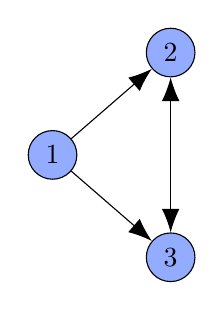
\begin{tikzpicture}[>={Latex[length=3mm]},auto, on grid]
      \node[nodeSBlue] (1) {$1$};
      \node[nodeSBlue] (2) [above right = 1.3cm and 1.5cm of 1] {$2$};
      \node[nodeSBlue] (3) [below right = 1.3cm and 1.5cm of 1] {$3$};
      \draw[->] (1) edge[] node {} (2);
      \draw[->] (1) edge[] node {} (3);
      \draw[<->] (2) edge[] node {} (3);
    \end{tikzpicture}
  }
  \hfill
  \subcaptionbox{A simple undirected graph.\label{fig:graph1:b}}%
    [.3\linewidth] {
    \centering
    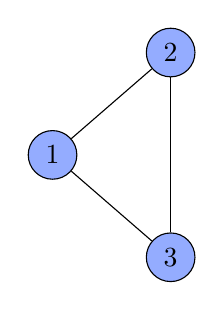
\begin{tikzpicture}[auto, on grid, ]
      \node[nodeSBlue] (1) {$1$};
      \node[nodeSBlue] (2) [above right = 1.3cm and 1.5cm of 1] {$2$};
      \node[nodeSBlue] (3) [below right = 1.3cm and 1.5cm of 1] {$3$};
      \draw[-] (1) edge[] node {} (2);
      \draw[-] (1) edge[] node {} (3);
      \draw[-] (2) edge[] node {} (3);
    \end{tikzpicture}
  }
  \hfill
  \subcaptionbox{An undirected multigraph.\label{fig:graph1:c}}%
    [.3\linewidth] {
    \centering
    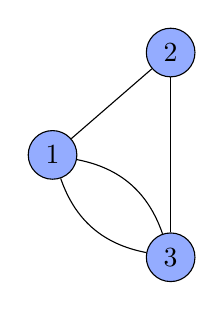
\begin{tikzpicture}[auto, on grid, ]
      \node[nodeSBlue] (1) {$1$};
      \node[nodeSBlue] (2) [above right = 1.3cm and 1.5cm of 1] {$2$};
      \node[nodeSBlue] (3) [below right = 1.3cm and 1.5cm of 1] {$3$};
      \draw[-] (1) edge[] node {} (2);
      \draw[-] (1) edge[bend left] node {} (3);
      \draw[-] (1) edge[bend right] node {} (3);
      \draw[-] (2) edge[] node {} (3);
    \end{tikzpicture}
  }
  \caption{Examples of different graphs}
  \label{fig:graph1}
\end{figure}

\emph{Undirected graph} is a graph in which the order of the vertices in an edge does not matter.
An edge of an undirected graph is defined as an unordered pair $\{v, w\} \in E$, therefore the following holds:
\begin{equation}
\forall v, w \in V\colon \{v, w\} = \{w, v\}
\end{equation}
For example $E=\{\{1, 2\}, \{1, 2\}, \{3, 2\}, \{2, 3\}, \{1, 3\}\}=\{\{1,2\},\{1,3\},\{2,3\}\}$.
Visualization of this graph $G=(\{1,2,3\}, E)$ can be seen in the Figure \ref{fig:graph1:b}.
For the purpose of this work, we need only undirected graphs.

The definitions of graphs shown earlier do not restrict an edge to start and end in itself ($e=(v, v)$).
This kind of an edge is called a \emph{loop}.
The definitions however restricts \emph{multiple edges} (identical parallel edges).
In order to allow multiple edges, the edge set has to be defined as a \emph{multiset}.
A graph that contains multiple edges is called a \emph{multigraph}.
Depending on the author or context, multigraphs either allow or disallow loops.
In this work, we consider multigraphs to exist without loops.

A graph that has no loops or multiple edges is called a \emph{simple graph}.
Simple graphs can either be directed or undirected and it should be explicitly mentioned when defining graphs, unless the context implies it.
As we do not need directedness of edges, let us assume that further expressions of graphs are always undirected in this work.

Suppose there is an edge $e=\{v,w\}$.
We say that vertex $v$ is \emph{incident} to $e$ and $e$ is incident to $v$.
We also say that vertex $v$ is \emph{adjacent} to $w$ and vice versa.
Similarly when two edges share a vertex, we say that the edges are \emph{adjacent}.
We can also say that $w$ is a \emph{neighbour} of $v$ and vice versa.

In a graph, the degree of a vertex is the number of edges it is incident to.
We will use the notation $\deg_G(v)$ to denote the degree of vertex $v \in V$ in graph $G=(V,E)$.
In multigraphs with loops, a loop counts as 2 to a degree.

A graph that is \emph{bipartite} has exactly two disjoint sets of vertices (we call them part $A$ and part $B$), and every edge of the graph has one endpoint in vertex of $A$ and another in $B$:
\begin{align}
V &= A \cup B\\
A \cap B &= \emptyset\\
E &=\{\{a, b\} \mid a \in A, b \in B\}
\end{align}
For bipartite graphs, the sum of degrees on $A$ and $B$ are equal:
\begin{equation}
\sum_{a\in A} \deg_G(a) = \sum_{b\in B} \deg_G(b)
\end{equation}
An example of a bipartite graph can be seen in Figure \ref{fig:graph2}.

\begin{figure}[H]
\centering
% https://tex.stackexchange.com/a/499577
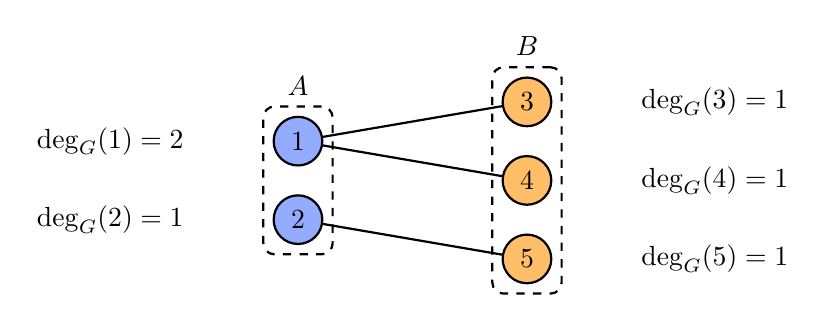
\begin{tikzpicture}[thick,amat/.style={matrix of nodes,nodes in empty cells,
  row sep=1em,draw,dashed,rounded corners,
  nodes={draw,solid,circle}},
  fsnode/.style={fill=strongBlue},
  ssnode/.style={fill=strongOrange}]

  \matrix[amat,nodes=fsnode,label=above:$A$] (mat1) {
  1\\
  2\\
  };

  \matrix[amat,right=2cm of mat1,nodes=ssnode,label=above:$B$] (mat2) {
  3\\
  4\\
  5\\};

  \node (1) [left = of mat1-1-1] {$\deg_G(1)=2$};
  \node (2) [left = of mat1-2-1] {$\deg_G(2)=1$};
  \node (3) [right = of mat2-1-1] {$\deg_G(3)=1$};
  \node (4) [right = of mat2-2-1] {$\deg_G(4)=1$};
  \node (5) [right = of mat2-3-1] {$\deg_G(5)=1$};
  \draw (mat1-1-1) edge (mat2-1-1);
  \draw (mat1-1-1) edge (mat2-2-1);
  %\draw (mat1-2-1) edge (mat2-2-1);
  \draw (mat1-2-1) edge (mat2-3-1);
\end{tikzpicture}
\caption{A simple disconnected bipartite graph.\label{fig:graph2}}
\end{figure}

If all vertices in a graph have the same degree, then the graph is called \emph{regular}.
For example, if every vertex in a bipartite graph shares a degree, then we call it a regular bipartite graph. When every node $a$ of part $A$ share a degree and every node $b$ of part $B$ share a degree, we call it \emph{a biregular graph}.
In fact, we use a notation $(d_A,d_B)$-biregular, where $d_A$ and $d_B$ denote the degrees of the nodes inside parts $A$ and $B$ respectively.
We can see an example of a (3,2)-biregular in Figure \ref{fig:graph3}.
The bipartite graph in Figure \ref{fig:graph2} is not biregular because the nodes in part $A$ do not share a degree i.e. for all nodes $v, w \in A$ the condition $\deg_G(v) = \deg_G(w)$ does not hold.

\begin{figure}[H]
\centering
% https://tex.stackexchange.com/a/499577
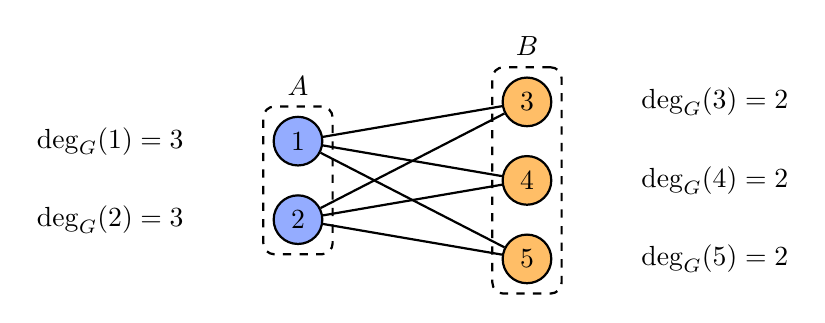
\begin{tikzpicture}[thick,amat/.style={matrix of nodes,nodes in empty cells,
  row sep=1em,draw,dashed,rounded corners,
  nodes={draw,solid,circle}},
  fsnode/.style={fill=strongBlue},
  ssnode/.style={fill=strongOrange}]

  \matrix[amat,nodes=fsnode,label=above:$A$] (mat1) {
  1\\
  2\\
  };

  \matrix[amat,right=2cm of mat1,nodes=ssnode,label=above:$B$] (mat2) {
  3\\
  4\\
  5\\};

  \node (1) [left = of mat1-1-1] {$\deg_G(1)=3$};
  \node (2) [left = of mat1-2-1] {$\deg_G(2)=3$};
  \node (3) [right = of mat2-1-1] {$\deg_G(3)=2$};
  \node (4) [right = of mat2-2-1] {$\deg_G(4)=2$};
  \node (5) [right = of mat2-3-1] {$\deg_G(5)=2$};
  \draw (mat1-1-1) edge (mat2-1-1);
  \draw (mat1-1-1) edge (mat2-2-1);
  \draw (mat1-1-1) edge (mat2-3-1);
  \draw (mat1-2-1) edge (mat2-1-1);
  \draw (mat1-2-1) edge (mat2-2-1);
  \draw (mat1-2-1) edge (mat2-3-1);
\end{tikzpicture}
\caption{A simple (3,2)-biregular graph.\label{fig:graph3}}
\end{figure}


A graph is considered as \emph{connected} if from every node one can traverse through the edges to all other nodes i.e. every pair of nodes need to also be connected.
For instance, the graph in Figure \ref{fig:graph2} has two isolated vertex subsets $\{2, 5\}$ and $\{1, 3, 4\}$, therefore the graph is \emph{disconnected}.
On the other hand, the graphs in Figures \ref{fig:graph1:b}, \ref{fig:graph1:c} and \ref{fig:graph3} are connected.
Let us not worry about the connectivity of the directed graph on Figure \ref{fig:graph1:a} as directed graphs are not relevant to this work other than in this section.

A \emph{distance} between two nodes $u, v\in V$ is the length of the shortest path between $u$ and $v$ (see Figure \ref{fig:graph4:b}).
We use the notation $\operatorname{dist}(u, v)$ for the distance between $u$ and $v$.
The maximum of all shortest paths in a graph $G$ is called the \emph{diameter} of $G$.
A \emph{subgraph} $H$ of a graph $G=(V, E)$ is a graph formed from a subset $V'$ of vertices of $V$ and a subset $E'$ of edges of $E$ such that each endpoint of $e' \in E'$ must be in $V'$.
A $r$-radius \emph{ball} of node $u$ of graph $G$ is a subgraph $H=(V', E')$ of $G$ containing:
\begin{itemize}
  \item every vertex $v\in V$ such that the distance from $u$ to $v$ is at most $r$,
  \item every edge $(u', v') \in E$ such that $u'$ and $v'$ are also in $V'$.
\end{itemize}
We use the notation $B_G(u, r)$ to denote the $r$-radius ball of node $u$ of graph $G$.
For an example of a ball, see the Figure \ref{fig:graph5}.

\begin{figure}[H]
  \subcaptionbox{A path between nodes 1 and 5 in a graph $G$.
  The length of the path is 4.
  \label{fig:graph4:a}}
    [.30\linewidth] {
    \centering
    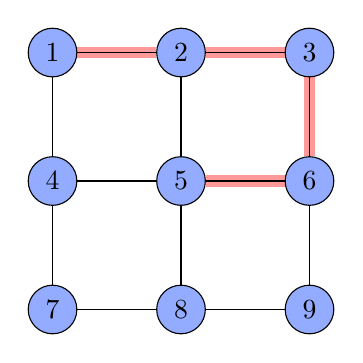
\begin{tikzpicture}[]
      \node[nodeSBlue] (1) [] at (0,0) {$1$};
      \node[nodeSBlue] (2) [right =  of 1] {$2$};
      \node[nodeSBlue] (3) [right =  of 2] {$3$};
      \node[nodeSBlue] (4) [below =  of 1] {$4$};
      \node[nodeSBlue] (5) [below =  of 2] {$5$};
      \node[nodeSBlue] (6) [below =  of 3] {$6$};
      \node[nodeSBlue] (7) [below =  of 4] {$7$};
      \node[nodeSBlue] (8) [below =  of 5] {$8$};
      \node[nodeSBlue] (9) [below =  of 6] {$9$};
      \draw[highlight] (1) -- (2);
      \draw[highlight] (2) -- (3);
      \draw[] (4) -- (5);
      \draw[highlight] (5) -- (6);
      \draw[] (1) -- (4);
      \draw[] (2) -- (5);
      \draw[highlight] (3) -- (6);
      \draw[] (4) -- (7);
      \draw[] (5) -- (8);
      \draw[] (6) -- (9);
      \draw[] (7) -- (8);
      \draw[] (8) -- (9);
    \end{tikzpicture}
  }
  \hfill
  \subcaptionbox{A shortest path between nodes 1 and 5 in a graph $G$.
  The length of the path is 2, thus $\operatorname{dist}(u,v)=2$.
  \label{fig:graph4:b}}
    [.30\linewidth] {
    \centering
    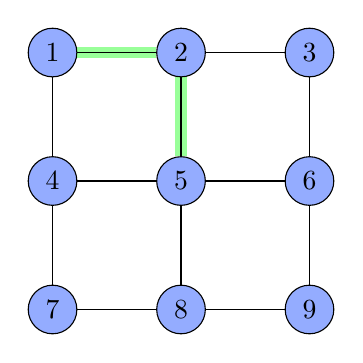
\begin{tikzpicture}[]
      \node[nodeSBlue] (1) [] at (0,0) {$1$};
      \node[nodeSBlue] (2) [right =  of 1] {$2$};
      \node[nodeSBlue] (3) [right =  of 2] {$3$};
      \node[nodeSBlue] (4) [below =  of 1] {$4$};
      \node[nodeSBlue] (5) [below =  of 2] {$5$};
      \node[nodeSBlue] (6) [below =  of 3] {$6$};
      \node[nodeSBlue] (7) [below =  of 4] {$7$};
      \node[nodeSBlue] (8) [below =  of 5] {$8$};
      \node[nodeSBlue] (9) [below =  of 6] {$9$};
      \draw[highlight={green}] (1) -- (2);
      \draw[] (2) -- (3);
      \draw[] (4) -- (5);
      \draw[] (5) -- (6);
      \draw[] (1) -- (4);
      \draw[highlight={green}] (2) -- (5);
      \draw[] (3) -- (6);
      \draw[] (4) -- (7);
      \draw[] (5) -- (8);
      \draw[] (6) -- (9);
      \draw[] (7) -- (8);
      \draw[] (8) -- (9);
    \end{tikzpicture}
  }
  \hfill
  \subcaptionbox{A path between nodes 1 and 9 illustrating the diameter of the graph $G$.
  The length of the path is 4, thus $\operatorname{diameter}(G)=4$.
  \label{fig:graph4:c}}
    [.30\linewidth] {
    \centering
    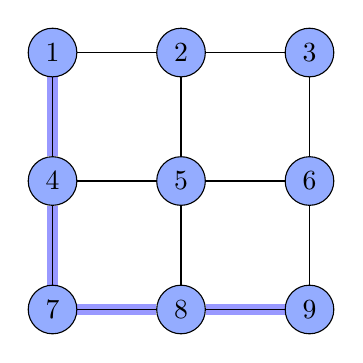
\begin{tikzpicture}[]
      \node[nodeSBlue] (1) [] at (0,0) {$1$};
      \node[nodeSBlue] (2) [right =  of 1] {$2$};
      \node[nodeSBlue] (3) [right =  of 2] {$3$};
      \node[nodeSBlue] (4) [below =  of 1] {$4$};
      \node[nodeSBlue] (5) [below =  of 2] {$5$};
      \node[nodeSBlue] (6) [below =  of 3] {$6$};
      \node[nodeSBlue] (7) [below =  of 4] {$7$};
      \node[nodeSBlue] (8) [below =  of 5] {$8$};
      \node[nodeSBlue] (9) [below =  of 6] {$9$};
      \draw[] (1) -- (2);
      \draw[] (2) -- (3);
      \draw[] (4) -- (5);
      \draw[] (5) -- (6);
      \draw[highlight={blue}] (1) -- (4);
      \draw[] (2) -- (5);
      \draw[] (3) -- (6);
      \draw[highlight={blue}] (4) -- (7);
      \draw[] (5) -- (8);
      \draw[] (6) -- (9);
      \draw[highlight={blue}] (7) -- (8);
      \draw[highlight={blue}] (8) -- (9);
    \end{tikzpicture}
  }
  \caption{Examples of different kind of paths illustrated by highlighting the edges that form the path.}
  \label{fig:graph4}
\end{figure}

\begin{figure}[H]
  \subcaptionbox{The graph $G$ from Figure \ref{fig:graph4}.
  Inside the red area is each node with distance at most 1 to node 5.
  \label{fig:graph5:a}}
    [.45\linewidth] {
    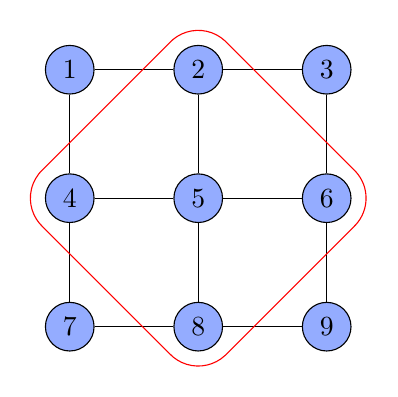
\begin{tikzpicture}[]
      \node[nodeSBlue] (1) [] at (0,0) {$1$};
      \node[nodeSBlue] (2) [right =  of 1] {$2$};
      \node[nodeSBlue] (3) [right =  of 2] {$3$};
      \node[nodeSBlue] (4) [below =  of 1] {$4$};
      \node[nodeSBlue] (5) [below =  of 2] {$5$};
      \node[nodeSBlue] (6) [below =  of 3] {$6$};
      \node[nodeSBlue] (7) [below =  of 4] {$7$};
      \node[nodeSBlue] (8) [below =  of 5] {$8$};
      \node[nodeSBlue] (9) [below =  of 6] {$9$};
      \draw[] (1) -- (2);
      \draw[] (2) -- (3);
      \draw[] (4) -- (5);
      \draw[] (5) -- (6);
      \draw[] (1) -- (4);
      \draw[] (2) -- (5);
      \draw[] (3) -- (6);
      \draw[] (4) -- (7);
      \draw[] (5) -- (8);
      \draw[] (6) -- (9);
      \draw[] (7) -- (8);
      \draw[] (8) -- (9);
      \draw[red] \convexpath{4,2,6,8}{0.5cm};
    \end{tikzpicture}
    }
    \hfill
    \subcaptionbox{A 1-radius ball $B_G(5, 1)$ is a subgraph of $G$.
    \label{fig:graph5:b}}
      [.45\linewidth] {
      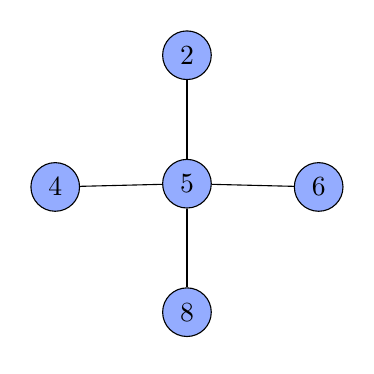
\begin{tikzpicture}[]
        \node[draw=none, minimum size=0.7cm] (1) [] at (0,0) {};
        \node[nodeSBlue] (2) [right =  of 1] {$2$};
        \node[draw=none, minimum size=0.7cm] (3) [right =  of 2] {};
        \node[nodeSBlue] (4) [below =  of 1] {$4$};
        \node[nodeSBlue] (5) [below =  of 2] {$5$};
        \node[nodeSBlue] (6) [below =  of 3] {$6$};
        \node[draw=none, minimum size=0.7cm] (7) [below =  of 4] {};
        \node[nodeSBlue] (8) [below =  of 5] {$8$};
        \node[draw=none, minimum size=0.7cm] (9) [below =  of 6] {};
        %\draw[] (1) -- (2);
        %\draw[] (2) -- (3);
        \draw[] (4) -- (5);
        \draw[] (5) -- (6);
        %\draw[] (1) -- (4);
        \draw[] (2) -- (5);
        %\draw[] (3) -- (6);
        %\draw[] (4) -- (7);
        \draw[] (5) -- (8);
        %\draw[] (6) -- (9);
        %\draw[] (7) -- (8);
        %\draw[] (8) -- (9);
        %\draw[red] \convexpath{4,2,6,8}{0.5cm};
      \end{tikzpicture}
      }
  \caption{Example of a ball.}
  \label{fig:graph5}
\end{figure}


\subsection{Distributed computing} \label{sec:distributed_computing}
Executing a computer program in several identical or different computers is called distributed computing
\cite{DBLP:books/el/leeuwen90/LamportL90}.
It is similar to running a computer program that contains multiple concurrent tasks, in a computer, but in distributed computing there are higher level tasks that are distributed to different computer nodes.

Computers are called nodes, and they are connected to each other with communication channels.
These communication channels carry data from a node to another node.
Together, nodes and communication channels form a network.
A common way to visualize these networks is by drawing a graph in which the nodes represent computing nodes and edges represent the communication channels.
\cite{HirvonenSuomelaDistAlg2020}


\begin{figure}[H]
  \subcaptionbox{A small distributed network containing 5 nodes.
    \label{fig:dist_comp1:a}
  }%
    [.45\linewidth] {
    \centering
  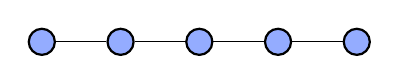
\begin{tikzpicture}[every node/.style={circle,thick,draw}]
    \node[nodeSBlue] (1) {};
    \node[nodeSBlue] (2) [ right of=1] {};
    \node[nodeSBlue] (3) [ right of=2] {};
    \node[nodeSBlue] (4) [ right of=3] {};
    \node[nodeSBlue] (5) [ right of=4] {};
    \draw (1) -- (2);
    \draw (2) -- (3);
    \draw (3) -- (4);
    \draw (4) -- (5);
  \end{tikzpicture}
  }
  \hfill
  \subcaptionbox{
    A larger distributed network containing 120 nodes.
    \label{fig:dist_comp1:b}
  }%
    [.45\linewidth] {
    \centering
  \resizebox{0.45\textwidth}{!}{%
  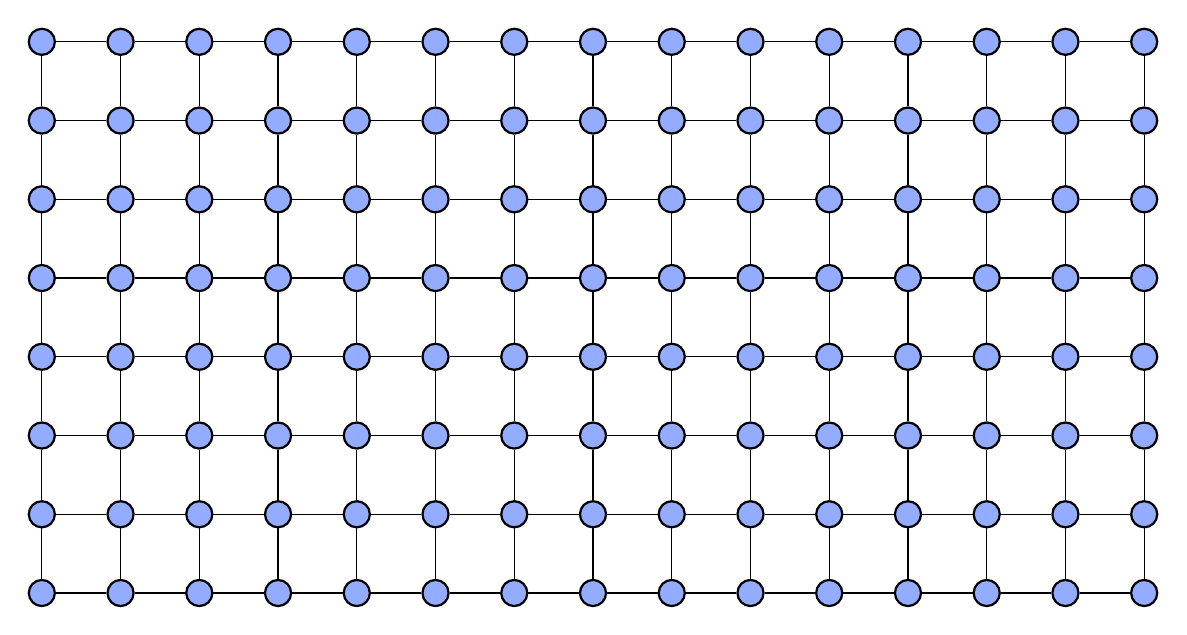
\begin{tikzpicture}[every node/.style={circle,thick,draw}]
    \pgfmathtruncatemacro{\maxX}{14}
    \pgfmathtruncatemacro{\maxY}{7}
    \pgfmathtruncatemacro{\maxXm}{\maxX - 1}
    \pgfmathtruncatemacro{\maxYm}{\maxY - 1}
    % Nodes
    \foreach \x in {0,...,\maxX}
      \foreach \y in {0,...,\maxY}
           \node [nodeSBlue]  (\x\y) at (\x,\y) {};
    % Vertical edges
    \foreach \x [count=\xi] in {0,...,\maxX}
      \foreach \y [count=\yi] in {0,...,\maxYm} {
        \draw (\x\y)--(\x\yi);
      }
    % Horizontal edges
    \foreach \x [count=\xi] in {0,...,\maxXm}
      \foreach \y [count=\yi] in {0,...,\maxY} {
        \draw (\x\y)--(\xi\y);
      }
  \end{tikzpicture}
  }%
%    \includegraphics[scale=0.4]{diagrams/dist_comp1.pdf}
    %\missingfigure{A bigger distributed network example}
  }
  \caption{Examples of distributed networks.}
  \label{fig:dist_comp1}
\end{figure}
According to Lamport \cite{DBLP:books/el/leeuwen90/LamportL90}, in the area of distributed computing, the term \emph{model} denotes a view or abstract representation of a distributed system.
There are multiple different computation models used in distributed computing \cite{DBLP:books/el/leeuwen90/LamportL90}.
The most important category of distributed computation models is \emph{process models} \cite{DBLP:books/el/leeuwen90/LamportL90}.
In process models, the work or activities are represented as concurrently executed processes that execute their instructions sequentially \cite{DBLP:books/el/leeuwen90/LamportL90}.
A standard way to distinguish different process models from each other is to categorise them by the method they use to communicate with each other (\emph{interprocess communication}) \cite{DBLP:books/el/leeuwen90/LamportL90}.


%\subsubsection{Message passing model} \label{sec:message_passing_model}
Message passing models are one form of a process model \cite{DBLP:books/el/leeuwen90/LamportL90}.
In the model, processes communicate by adding a message to a message queue, and the recipient process moves the message out (dequeues) from the message queue \cite{DBLP:books/el/leeuwen90/LamportL90}.

Different message passing models are widely used in the research field of distributed computing.
The models can vary in different details, such as in the size of the message queues \cite{DBLP:books/el/leeuwen90/LamportL90}, in the size of the messages \cite{peleg2000distributed} and on how the nodes get identified \cite{DBLP:conf/focs/Linial87}, if they are identified at all \cite{DBLP:conf/istcs/MayerNS95}.
%As the message passing models itself can be defined in multiple ways \cite{DBLP:books/el/leeuwen90/LamportL90}, we will use a definition from which the relevant models commonly inherit from.
We will dive deeper into the most relevant message passing models for this work in Sections \ref{sec:port_number_model} and \ref{sec:local_model}.

An algorithm that is executed in a distributed fashion in a distributed network, is called as a distributed algorithm.
Each node in a network is started simultaneously and will always execute the same algorithm.
Initially the nodes are on the same state and there can be finitely or infinitely many states.
Initially the nodes are aware of only themselves and of the connections to their neighbours.
One might question that if every node starts with the same state, would not they also end up in the same state?
Well yes, this happens inevitably in a case where the nodes were not given any additional symmetry breaking inputs and if every node sees the same amount of neighbours \cite{HirvonenSuomelaDistAlg2020}.

%For example, we have a chain like network $W$ where each node $w$ has exactly two neighbours.
%The task is to execute an algorithm that finds the number of nodes in the network.


In practice, every computer node on a network has an UUID (Universally unique identifier) that can be used to break the symmetry, and nodes are usually given some input data that they process, and nodes can always randomize data as they are never completely synchronized together, so this is not necessarily a problem.
In theory, we explicitly have to assume that there exists these kind of symmetry breaking elements.
In this works, distributed algorithms are deterministic unless otherwise mentioned.
In other research there might be randomizing involved.


%TODO Find a correct place to talk  about execution times if there is any}
%In the message passing model, one could easily think that the execution time of the algorithm is the standard unit used to measure the performance but this is not true.
%The message passing model implies that the dominant cost during an execution of a distributed algorithm is the message passing itself
%\cite{DBLP:books/el/leeuwen90/LamportL90}.
%This really...
%TODO continue here




%The following two sections (\ref{sec:port_number_model} and \ref{sec:local_model} ) talk about different forms of message passing models that are highly relative to this paper.

\subsection{Port number model} \label{sec:port_number_model}
This section is based on the excellent textbook \cite{HirvonenSuomelaDistAlg2020} unless otherwise mentioned.

Port number model (PN model) is a rather weak model of computation that inherits from the message passing model.
In the model, nodes do not have identification.
A distributed algorithm that executes in a port number model is called as a PN-algorithm.

%We can basically take any network $N$ that has the same structure as a simple undirected graph $G$.
%Each vertex of $G$ can be one-to-one mapped (bijection) to the nodes of $N$ and vice-versa.
%Respectively all edges $(v, w)$ of $G$ can be mapped to communication channels between nodes $v$ and $w$.

Communication channels start and end from communication ports.
Each node has communication ports numbered from $1$ to $d$, where $d$ is the degree of the node.
The ports are numbered in an arbitrary order.

All nodes are considered identical; initially they are in the same internal state.
Every node starts the execution simultaneously following the same PN-algorithm $A$.
The execution of $A$ is done synchronously in parallel.
A communication round consists of following synchronous steps:
\begin{enumerate}
  \item send a message to each port,
  \item wait until all messages have been sent,
  \item receive a message from each port,
  \item update internal state.
\end{enumerate}
After each communication round, a node can optionally stop execution and announce its local output.
All nodes are required to eventually stop.
When all nodes have stopped, the algorithm is considered as stopped.
The running time of the algorithm $A$ is the total communication rounds that took place.


\subsection{Formalized port number model} \label{sec:formalized_pn_model}
In Section \ref{sec:port_number_model} we briefly and informally introduced the PN model.
Now in this section and in the following subsections we give a more formal definition to the PN model.
As in the previous section, this section is based on the textbook \cite{HirvonenSuomelaDistAlg2020} unless otherwise mentioned.

PN network is a 3-element tuple $N = (V, P, p)$, where $V$ and $P$ are the sets of vertices and ports respectively, and $p\colon P \rightarrow P$ is a function that maps a port to another port, forming a communication channel.
A port, an element of $P$, is a pair $(v, i)$ where $v \in V$ and $i \in \{1, 2, \dotsc\}$.
Additionally we assume that $p$ is an involution, that is, for all ports $x \in P$ we have $p(p(x)) = x, $ i.e. each edge of the ``underlying graph'' is undirected.
See Figures \ref{fig:formal_pn1:a} and \ref{fig:formal_pn1:b} for examples of valid and invalid PN networks.

\begin{figure}[H]
  \subcaptionbox{A PN network of two nodes, $a$ and $b$.
    Both $a$ and $b$ have degree of 2, therefore 2 ports.
    Ports are $(a, 1), (a, 2), (b, 1)$ and $(b, 2)$.
    The connections are
      $p((a, 1)) = (b, 1)$,
      $p((a, 2)) = (b, 2)$,
      $p((b, 1)) = (a, 1)$ and
      $p((b, 2)) = (a, 2)$.
    \label{fig:formal_pn1:a}
  }%
    [.45\linewidth] {
    \centering
    \includegraphics[scale=0.6]{diagrams/formalizing_pn_network_diagram1.pdf}
  }
  \hfill
  \subcaptionbox{
    An invalid PN network as port mapping function $p$ is not an involution:
    $p(p((a, 1))) = p(p((a, 2))) \neq (a, 1)$.
    \label{fig:formal_pn1:b}
  }%
    [.45\linewidth] {
    \centering
    \includegraphics[scale=0.6]{diagrams/formalizing_pn_network_diagram2.pdf}
  }
  \caption{Examples of a valid and an invalid PN network.}
  \label{fig:formal_pn1}
\end{figure}


The degree $\deg_N(v)$ of a node $v \in V$ is equal to the number of ports of $v$.
We assume that the port numbers are consecutive positive integers starting from 1, i.e. the ports of a node $v$ are $\{(v, i) \mid i \in \{1, 2, \dotsc, \deg_N(v)\}\}$.
Note that the highest port number of $v$ is also the degree of $v$.

When we say \emph{port number $i$ in node $v$}, we refer to the port $(v, i)$.
When we say \emph{port $(v, i)$ is connected to port $(w, j)$}, we refer to $p((v, i)) = (w, j)$.

A loop is a connection where port $(v, i)$ is connected to port $(v, j)$.
For example there are two loops, $p((a, 1)) = (a, 2)$ and $p((c,2)) = (c,2)$, in Figure \ref{fig:formal_pn2:c}.

There are multiple connections between two distinct nodes $v$ and $w$ if $p((v, i_1)) = (w, j_1)$, $p((v, i_2)) = (w, j_2)$, $i_1 \neq j_1$ and $i_2 \neq j_2$.
For example there are connections $p((b, 2)) = (d, 1)$ and $p((b, 3)) = (d, 2)$ in Figure \ref{fig:formal_pn2:c}.

If a PN network has neither loops or multiple connections, it is called a \emph{simple} PN network.
For example the network is simple in Figure \ref{fig:formal_pn2:a}.


\begin{figure}[H]
  \subcaptionbox{
    A simple PN network.
    The underlying graph is also simple.
    \label{fig:formal_pn2:a}
  }%
    [.3\linewidth] {
    \centering
    \includegraphics[scale=0.55]{diagrams/formalizing_pn_network_diagram4.pdf}
  }
  \hfill
  \subcaptionbox{
    An alternative representation of the PN network from Figure \ref{fig:formal_pn2:b}
    \label{fig:formal_pn2:b}
  }%
    [.3\linewidth] {
    \centering
    \includegraphics[width=0.3\textwidth]{diagrams/formalizing_pn_network_diagram5.pdf}
  }
  \hfill
  \subcaptionbox{
    A PN network with loops and parallel connections.
    This kind of network cannot be shown in the alternative representation unlike the network on Figure \ref{fig:formal_pn2:a}.
    \label{fig:formal_pn2:c}
  }%
    [.3\linewidth] {
    \centering
    \includegraphics[scale=0.55]{diagrams/formalizing_pn_network_diagram3.pdf}
  }
  \caption{Examples of simple and non simple PN networks.}
  \label{fig:formal_pn2}
\end{figure}


\subsubsection{Underlying graph} \label{sec:underlying_graph}

Each simple PN network $N=(V,P,p)$ has an \emph{underlying graph} $G=(V,E)$.
An edge $\{v, w\}$ is part of the underlying network $G$ if and only if $v$ is connected to $w$, that is, $E = \{ \{v, w\} \mid  p((v, i)) = (w, j) \}$.
A network with multiple connections uses the same definition to determine an underlying network, but in that case $E$ has to be a multiset instead of a set, in order to allow multiple same edges.

In case an underlying graph of a network is connected, we say that \emph{the network is connected.}
Throughout this work, we assume that the introduced networks are connected.

\begin{figure}[H]
  \subcaptionbox{
    An underlying simple graph of the simple PN network from Figure \ref{fig:formal_pn2:a} and Figure \ref{fig:formal_pn2:b}.
    \label{fig:underlying_graphs1:a}
  }%
    [.45\linewidth] {
    \centering
    \includegraphics[scale=0.6]{diagrams/formalizing_pn_network_underlying_graph_1.pdf}
  }
  \hfill
  \subcaptionbox{
    An underlying multigraph of the PN network with multiple connections in Figure \ref{fig:formal_pn1:a}.
    \label{fig:underlying_graphs1:b}
  }%
    [.45\linewidth] {
    \centering
    \includegraphics[width=0.3\textwidth]{diagrams/formalizing_pn_network_underlying_graph_2.pdf}
  }
  \caption{Examples of underlying graphs.}
  \label{fig:underlying_graphs1}
\end{figure}

%\subsubsection{Node labelings}
\subsubsection{Distributed graph problems} \label{sec:dist_graph_probl}
Researchers are often interested in different distributed graph problems.
These problems always have some kind of set of solution.
As it turns out, many of these problems can be encoded using the node labelings.

%TODO feels like this needs a smooth transition from the previous topic
Node labelings are a way to associate information with each node $v \in V$.
It is defined as a function $f\colon V \rightarrow Y$, where $Y$ is an arbitrary set of labels.

We can use the concept of node labelings to represent subsets $X_1, X_2, \dotsc, X_n \in V$ for some $n \in \mathbb{Z}_{>0}$ with node labeling $g\colon V \rightarrow \{1, 2, \dotsc, n\}$ where $g(v) = i$ indicates that $v \in X_i$ and $v \notin X_j, j \neq i$.
Note that the subsets $X_1, X_2, \dotsc, X_n$  are disjoint, and $X_1 \cup X_2 \cup \dotsb \cup X_n = V$.

Let $\Pi$ be a distributed graph problem.
The value of $\Pi(N)$ is the set of solutions, where $N=(V, P, p)$ is a simple PN network.
A solution $f \in \Pi(N)$ is a node labeling $f\colon V \rightarrow Y$, where $Y$ is some set of local outputs specific to the problem in question.

%Next we will give some examples of distributed graph problems and what kind of node labelings their solutions have.
For example:
\begin{description}
  \item[Vertex cover] of a graph $G$ is a subset $V' \subseteq V$ of nodes which together \emph{cover} all edges of the graph, that is, at least one endpoint from each edge must be in the subset $V'$.
  A node labeling $f$ is a solution $f \in \Pi(N)$ if $f$ encodes a vertex cover of the underlying graph $G$ of $N$.
  \item[Independent set] of a graph $G$ is a subset $V' \subseteq V$ of nodes where no two nodes are adjacent. That is, for each $u, v, \in V' s.t. u \neq v$, an edge $(u, v)$ is not in $E$.
  A node labeling $f$ is a solution $f \in \Pi(N)$ if $f$ encodes an independent set of nodes of the underlying graph $G$ of $N$.
  \item[Maximal independent set] of a graph $G$ is an independent subset $V' \subseteq V$ of nodes such that there is no additional vertex $w \in V \backslash V'$ that can be included in $V'$ such that it stays as an independent set.
  A node labeling $f$ is a solution $f \in \Pi(N)$ if $f$ encodes an independent set of nodes of the underlying graph $G$ of $N$.
  \item[$k$-coloring] of a graph $G$ is partition of $V$ with $k$ subsets $X_1, X_2, \dotsc, X_k$ where each subset is an independent set.
  A node labeling $f$ is a solution $f \in \Pi(N)$ if $f$ encodes a $k$-coloring of the underlying graph $G$ of $N$.
\end{description}

In the first three problems it seems like we are looking for only one subset of vertices $V' \subseteq V$.
Indeed, but we also have the subset of vertices $V \backslash V'$, thus $n=2$.
Therefore we can define $X_1 = V'$ and $X_2 = V \backslash V'$.
In the problem $k$-coloring, we are looking for $k$ subsets of vertices $X_1, X_2, \dotsc, X_k$, therefore $n=k$.

\begin{figure}[H]
  \subcaptionbox{
    A vertex cover.
    \label{fig:distributed_graph_problems1:a}
  }%
    [.30\linewidth] {
    \centering
    \includegraphics[width=0.30\textwidth]{diagrams/formalizing_pn_network_6.pdf}
  }
  \hfill
  \subcaptionbox{
    A maximal independent set.
    \label{fig:distributed_graph_problems1:b}
  }%
    [.30\linewidth] {
    \centering
    \includegraphics[width=0.30\textwidth]{diagrams/formalizing_pn_network_7.pdf}
  }
  \hfill
  \subcaptionbox{
    A 3-coloring.
    \label{fig:distributed_graph_problems1:c}
  }%
    [.30\linewidth] {
    \centering
    \includegraphics[width=0.30\textwidth]{diagrams/formalizing_pn_network_8.pdf}
  }
  \caption{Example solutions to different graph problems.
  In Figures \ref{fig:distributed_graph_problems1:a} and \ref{fig:distributed_graph_problems1:b}, the blue nodes form a node labeling that denote a solution.
  In Figure \ref{fig:distributed_graph_problems1:c} there are two additional labels, yellow and green in order there to be 3 labels for 3 colors.
  }
  \label{fig:distributed_graph_problems1}
\end{figure}

In Figure \ref{fig:distributed_graph_problems1} we can see two examples of graph problem encodings.
The node labeling in Figure \ref{fig:distributed_graph_problems1:a} is a vertex cover.
However, the node labeling in Figure \ref{fig:distributed_graph_problems1:b} is not a vertex cover, because there is an edge $(d, f)$ and neither of the nodes are in the solution set $\{c, e\}$.
The node labeling in Figure \ref{fig:distributed_graph_problems1:b} is a maximal independent set.
On the other hand, the node labeling in Figure \ref{fig:distributed_graph_problems1:a} is not an independent set, because there is an edge $(e, f)$ and both $e$ and $f$ are in the solution set.



\subsubsection{Distributed algorithms in the PN model}

\newcommand{\algin}{\operatorname{Input}}
\newcommand{\algstates}{\operatorname{States}}
\newcommand{\algout}{\operatorname{Output}}
\newcommand{\algmsg}{\operatorname{Msg}}

\newcommand{\alginit}{\operatorname{init}}
\newcommand{\algsend}{\operatorname{send}}
\newcommand{\algrecv}{\operatorname{receive}}

A \emph{distributed algorithm} $A$ can be described as a state machine.
The algorithm $A$ can possibly have infinitely many states or only finitely many states.
The components of $A$ are:
\begin{enumerate}
  \item $\algin_A$ is the set of local inputs,
  \item $\algstates_A$ is the set of states,
  \item $\algout_A \subseteq \algstates_A$ is the set of states that are considered as output states,
  \item $\algmsg_A$ is the set of messages.
\end{enumerate}

The algorithm always consists of 3 functions, each defined for each degree $d \in \mathbb{N}$.
The first function, $$\alginit_{A,d}\colon \algin_A \rightarrow \algstates_A$$ initializes the state of the calling node using the given input data.
%The degree $d$ is also parameterized into the function meaning that the function can operate differently with different degree nodes.
Each node calls the function $\alginit_{A,d}$ as its first function call.

After initialization, each node constructs messages for each of their neighbour by calling the second function:
$$\algsend_{A,d}\colon \algstates_A \rightarrow \algmsg_A^d$$
A node gives its current local state as an input to the function and the returning value is a $d$-element tuple of messages.

The third function allows nodes to receive messages from each of their neighbours.
It is defined as:
$$\algrecv_{A,d}\colon \algstates_A \times \algmsg_A^d \rightarrow \algstates_A$$
The function is given a node's current state and a $d$-element tuple of received messages.
In return, it gives a state value that represents the node's new state.
Additionally whenever the current state is an output state $x \in \algout$, we require that the function $\algrecv_{A,d}$ returns the exact same state $x$.

\subsubsection{Execution of PN algorithm}

As formerly mentioned, a distributed algorithm $A$ can be described as a state machine.
Correspondingly the \emph{execution} of $A$ can be described as the history of states of each node of a PN network $N=(V, P, p)$.
Let $f\colon V \rightarrow \algin_A$ be a node labeling.
A \emph{state vector} is a function $x\colon V \rightarrow \algstates_A$.
The execution of $A$ on $(N, f)$ is a sequence of state vectors $x_0, x_1, \dotsc$ where the $x_0$ is the initial state vector.
When we use the notation $x_t, t \in \mathbb{Z}_{\geq 0}$, we refer to the state vector at time $t$.
Similarly, we use $x_t(u), u \in V$ when we refer to the state of the node $u$ at time $t$.

We define $$x_0(u) = \alginit_{A,d}(f(u))$$ where $u\in V$ and $d=\deg_N(u)$.
The state vectors $x_1, x_2, \dotsc$ are defined recursively in the following paragraph.

We assume that we have defined $x_{t-1}$ and we show how we define $x_{t}$ using the assumption of $x_{t-1}$.
Let function $m_t\colon P \rightarrow \algmsg_A$ map a port to a message at time $t$.
Let port $(v, j) \in P$, port $(u, i) = p((v, j))$, and degree $\deg_N(v) = d'$.
Let $m_t((u, i))$ be $j$'th element of the vector $\algsend_{A, d'}(x_{t-1}(v))$.
Here the element $m_t((u, i))$ is a message sent by node $v$ through communication port $(v, j)$.
It is also the message received by node $u$ from port $(u, i)$.

We define the message vector $$r_t(u)=(m_t((u, 1)), m_t((u, 2)), \dotsc, m_t((u, \deg_N(u))))$$ for each $u\in V$.
The message vector contains every message node $u$ receives at time~$t$.

Now we give the final definition for $x_t(u)$:
$$x_t(u) = \algrecv_{A,d}(x_{t-1}(u, r_t(u)))$$

Next we define when the execution is considered as stopped, using the definition of execution.
Algorithm \emph{$A$ stops in time $T$}, if $x_T(u) \in \algout_A$ for each $u \in V$, that is, each node $u$ is in output state at time $T$.
Algorithm \emph{$A$ stops}, if $A$ stops in some finite time $T$.


Now that we know when $A$ stops, we define what is considered as the output of $A$.
Assuming that $A$ stops in time $T$, we define the \emph{output} of $A$ as $g=x_T$.
With the same assumption, we define the \emph{local output} of node $u$ as $x_t(u)$.



\todo{Add an example execution of an example problem if necessary.} %TODO Add an example execution of an example problem if necessary.

\subsubsection{Solving graph problems in PN}
As this thesis focuses strongly on graph problems, it is necessary to define what it means for a distributed algorithm to solve a graph problem.

A family of graphs is a set of graphs with same kind of properties.
For example a set of all simple undirected graphs is a family of graphs.

Let $\mathcal{F}$ be a family of simple undirected graphs.
We assume that $N=(V, P, p)$ is a simple PN network, the underlying graph $G$ of $N$ is in the family $\mathcal{F}$ and finally the input $f$ to the algorithm $A$ is in $\Pi'(N)$.
We say that a distributed algorithm $A$ solves a problem $\Pi$ on a graph family $\mathcal{F}$ given problem $\Pi'$, if the execution of $A$ on $(N, f)$ stops and yields an output $g \in \Pi(N)$.
We say that $A$ solves the problem in time $T$, if $A$ stops in time $T(|V|)$ where $T\colon \mathbb{N} \rightarrow \mathbb{N}$.

The input problem $\Pi'$ is often omited.
Then we say that a distributed algorithm $A$ solves a problem $\Pi$ on a graph family $\mathcal{F}$.

Often when we discuss about some algorithms solving some problems, we state $\mathcal{F}, \Pi, \Pi'$ and $T$ implicitly.
For example \emph{algorithm $A$ finds a vertex cover in any bipartite graph} implies that $\mathcal{F}$ is bipartite graphs, $\Pi$ is the problem of finding a vertex cover and problem $\Pi'$ is omitted.

\todo{Continue from here with an example problem and an algorithm that solves it in some graph family given some other problem or omit it.}


\subsection{Covering map}
There exists a limitation to what problems can be solved in a deterministic PN model.
The limitation comes from an underlying graph of a PN network being symmetric~%
\cite{DBLP:conf/focs/Linial87}~%
\cite{DBLP:journals/siamcomp/Linial92}.

In this section we discuss about a topological concept that can help us formalizing symmetries in a PN network.
The concept is called \emph{covering map}
\footnote{Note that this is not related to the vertex cover problem even though they share the word \emph{cover}.}.
Later in this work, we use the concept in proving Theorems \ref{thm:lcl_nonsolvability:2} and \ref{thm:lcl_nonsolvability:3}.
%TODO Final check: are they all of the theorems where covering map is used?

First we want to show a definition of \emph{covering} for graphs from the paper
\cite{DBLP:conf/stoc/Angluin80}:
\begin{displayquote}
A graph $H$ is a \emph{covering} of a graph $G$ if there is a way to label the nodes of $H$ with the names of nodes in $G$ in such a way that if a node $x$ of $H$ is labelled ``v'' then the labels of the neighbors of $x$ are precisely the neighbors of $v$ in G.
\end{displayquote}
In this definition, covering map is the function that maps the nodes from $H$ to $G$.
If $H$ is a covering of a connected graph $G$, then an intuition is that $H$ consists of multiple copies of $G$ ``glued'' together in a clever way.


% First we define function $\xi_G(v)$ to be the set of all neighbors of vertex $v$ in graph $G$.
% If graphs $G=(V, E)$ and $G'=(V', E')$ are from the same graph family $\mathcal{F}$, we say that $G$ is a \emph{covering} of $G'$ via a map $\psi$ if and only if all of the following hold:
% \begin{enumerate}
%   \item $\psi=\psi: V \rightarrow V'$ such that for all vertices $v \in V$, the neighbour nodes $\xi_G(v)$ and $\xi_{G'}(\psi(v))$ are equal.
%   \item asd
% \end{enumerate}
In order for us to use covering maps with PN networks, we need to additionally consider the port numbers of nodes so that they are also preserver by the covering map.

We define now the covering map for PN networks similarly it is defined in the textbook \cite{HirvonenSuomelaDistAlg2020}.

\begin{definition} \label{def:covering_map}
  Let $N=(V, P, p)$ and $N'=(V', P', p')$ be PN networks and let $\phi\colon V \rightarrow V'$.
  The function $\phi$ is a covering map from $N$ to $N'$ if all of the following hold:
  \begin{enumerate}
    \item $\phi$ is a surjection i.e. for every $v' \in V'$ there exists at least one $v \in V$ such that $\phi(v) = v'$.
    \item $\phi$ preserves the degrees of a node i.e. $\deg_N(v) = \deg_{N'}(\phi(v))$, for all $v \in V$.
    \item $\phi$ preserves port numbers and connections i.e.\ if $p((u, i)) = (v, j)$ then $p'((\phi(u), i)) = (\phi(v), j)$.
  \end{enumerate}
\end{definition}

\begin{figure}[H]
  \subcaptionbox{
    A PN network N.
    \label{fig:covering_map1:a}
  }%
    [.5\linewidth] {
    \centering
    \includegraphics[scale=0.55]{diagrams/covering_map_1.pdf}
  }
  \hfill
  \subcaptionbox{
    A PN network N'.
    \label{fig:covering_map1:b}
  }%
    [.5\linewidth] {
    \centering
    \includegraphics[scale=0.55]{diagrams/covering_map_2.pdf}
  }
  \caption{There is a covering map $\phi$ from $N$ to $N'$ that maps each $x_i$ to $x$ for all $x\in \{a, b, c, d\}$ and for all $i \in \{1, 2\}$.
  }
  \label{fig:covering_map1}
\end{figure}

\begin{figure}[H]
  \subcaptionbox{
    A PN network N.
    \label{fig:covering_map2:a}
  }%
    [.5\linewidth] {
    \centering
    \includegraphics[scale=0.55]{diagrams/covering_map_3.pdf}
  }
  \hfill
  \subcaptionbox{
    A PN network N'.
    \label{fig:covering_map2:b}
  }%
    [.5\linewidth] {
    \centering
    \includegraphics[scale=0.55]{diagrams/covering_map_4.pdf}
  }
  \caption{There is a covering map $\phi$ from $N$ to $N'$ that maps each $a_i$ to $a$ for all $i \in \{1, 2, 3, 4\}$.
  }
  \label{fig:covering_map2}
\end{figure}

There are two examples of covering maps on Figure \ref{fig:covering_map1} and \ref{fig:covering_map2}.
In these examples we can see that the sizes of covering networks are integer multiplications of the sizes of original networks.
This actually
\footnote{\todo{Do I need to show this?}}
applies to every covering map, i.e. if we have a covering map $\phi\colon V \rightarrow V'$, then $|V| = k|V'|$ for some $k \in \mathbb{N}_{>0}$ \cite{DBLP:journals/dm/GrossT77}.
We often call covering networks as \emph{lifts}.
A \emph{$k$-lift} is a lift where the covering network $N$ is $k$ times the size of $N'$.




\begin{figure}[H]
  \subcaptionbox{
    A PN network $N_0$ with loops.
    \label{fig:covering_map3:a}
  }%
    [.30\linewidth] {
    \centering
    \includegraphics[scale=0.50]{diagrams/covering_map_5a.pdf}
  }
  \hfill
  \subcaptionbox{
    A PN network $N_1$ with multiple connections.
    \label{fig:covering_map3:b}
  }%
    [.30\linewidth] {
    \centering
    \includegraphics[scale=0.48]{diagrams/covering_map_5b.pdf}
  }
  \hfill
  \subcaptionbox{
    A simple PN network $N_2$.
    \label{fig:covering_map3:c}
  }%
    [.30\linewidth] {
    \centering
    \includegraphics[scale=0.46]{diagrams/covering_map_5c.pdf}
  }
  \caption{
    There is a covering map $\phi_0$ from $N_1$ to $N_0$ that maps each $x_i$ to $x$ for all $x \in \{a, b, c\}$ and for all $i \in \{1, 2\}$.
    Similarly there is a covering map $\phi_1$ from $N_2$ to $N_0$ that maps each $x_i$ to $x$ for all $x \in \{a, b, c\}$ and for all $i \in \{1, 2, 3\}$.
  }
  \label{fig:covering_map3}
\end{figure}

In the Figure \ref{fig:covering_map3} we can see that the network $N_1$ is a 2-lift of the network $N_0$ and the network $N_2$ is a 3-lift of the network $N_0$.
The network $N_0$ has 2 loops, $p(p((a, 2))) = p((a, 3)) = (a, 2)$ and $p(p((b, 2))) = p((b, 3)) = (b, 2)$.



%\todo{explain lift}
%\begin{figure}[H]
%  \centering
%  \includegraphics[]{example-image-duck}
%  \caption{Show lift from N' to N}
%  \label{fig:duck2}
%\end{figure}
%%%This implies that the graphs $H$ and $G$ are indistinguishable from a PN algorithm's perspective.
%%%\cite{DBLP:conf/stoc/Angluin80}

% Let $H=(V', E')$ and $G=(V, E)$ be some graphs in the graph family $\mathcal{F}$.
% A covering map is a function $\Phi: V' \rightarrow V$ that maps the vertices $v' \in V'$ to vertices $v \in V$ in such a way that if

%The function that maps $H$ to $G$ is called a \emph{covering map}.

This symmetricity implies that each node ends up in an identical output state with its symmetrical equivalent given that the input problem $\Pi$ does not break the symmetry.
% In this section we are discussing about a graph theoretic method that can show

continue...........

\subsection{LOCAL model} \label{sec:local_model}
The LOCAL model is another message passing model that is used in the field of distributed computation.
It inherits from the PN model, hence most of the definition is already done in Section \ref{sec:formalized_pn_model}.
The difference is that the graph problem $\Pi'$, given as an input, is always predetermined.
A solution to problem $\Pi'$ is a node labeling $\operatorname{id}\colon V \rightarrow \{1,2,\dotsc,|V|\}$, where each node has a unique label \cite{DBLP:conf/focs/Linial87}.
Sometimes the node labeling is defined $\operatorname{id}\colon V \rightarrow \{1,2,\dotsc,|V|^c\}$, where $c$ is a positive constant greater than 1 \cite{HirvonenSuomelaDistAlg2020}, but in this work we assume $c=1$.
If a distributed algorithm $A$ solves a problem $\Pi$ on a graph family $\mathcal{F}$ given $\Pi'$, we say that $A$ solves $\Pi$ on graph family $\mathcal{F}$ in the LOCAL model \cite{HirvonenSuomelaDistAlg2020}.

Earlier in Section \ref{def:covering_map} we discussed about the limitation in a deterministic PN model that comes from symmetry.
In the LOCAL model, an algorithm can utilize these identifiers to break the symmetry and avoid the limitation of the PN model.

A well-known property of the LOCAL model is the ability to compute \emph{every} function of a graph $G$ in time $\mathcal{O}(\operatorname{diameter}(G))$.
This amount of time is enough for any node in $G$ to gather complete information of both the graph and the unique labels from function $\operatorname{id}$, because a message can travel from a node to any other node at most in $\operatorname{diameter}(G)$ time.
With the complete information of everything, each node can compute the whole solution and output its own part of the solution.
Because of this, researchers are usually interested in complexity classes below the $\mathcal{O}(\operatorname{diameter}(G))$.

\todo{Discuss more about LOCAL? }

\subsection{Locally checkable labeling problems} \label{sec:lcl_problems}
In this section we define \emph{Locally checkable labeling (LCL)} problems generally.
This section is intended as an introduction for the Section \ref{sec:lcl_problems:biregular} where we introduce an alternative definition of LCL problems that we will be using in this work.
Briefly, LCL problems are a family of graph problems where a global solution (node labeling) can be verified locally by the individual nodes.


%TODO move this commented paragraph to somewhere where we talk about locality and complexity.
%LCL problems were first introduced in the paper \cite{DBLP:journals/siamcomp/NaorS95} by Moni Naor and Larry Stockmeyer in 1995.
%The paper laid the groundwork for further researches of the locality of distributed graph problems.
%\emph{Locality} is the maximum distance each node has to gather information from, in order to choose an output \cite{DBLP:journals/sigact/Suomela20}.
%Instead of discussing about locality, we can equally talk about round complexity of message passing algorithms \cite{DBLP:journals/sigact/Suomela20}.
%\todo{talk something about the constant radius and every t-time problem basically has to form the output based on the t-radius neighourhood (the information about the t-radius network the nodes have gathered) }.

\newcommand{\Sigmain}{\Sigma_{\text{in}}}
\newcommand{\Sigmaout}{\Sigma_{\text{out}}}


Now we define LCL problems using the formalism from the paper \cite{DBLP:journals/siamcomp/NaorS95} and we also use the formalism from a more recent paper \cite{DBLP:journals/corr/abs-2105-05574}.
An LCL problem $\Pi$ consists of:
\begin{itemize}
  \item a positive integer $r$, which is called the \emph{radius} of $\Pi$,
  \item a finite set of \emph{input labels} $\Sigmain$,
  \item a finite set of \emph{output labels} $\Sigmaout$ and
  \item a finite set of \emph{locally consistent labelings} $C$, where:
  \begin{itemize}
    \item the elements are pairs $(H=(V^H, E^H), s)$,
    \item $H$ is a graph, node $s$ is in $V^H$, and the distance from the node $s$ to any other node in $V^H$ is at most $r$,
    \item every pair $(v, e) \in (V^H \times E^H)$ is labeled with a pair from $\Sigmain \times \Sigmaout$.
  \end{itemize}
\end{itemize}
Given a graph $G = (V, E)$ and a node labeling $f: V \rightarrow \Sigmain \times \Sigmaout$, the node labeling $f$ is a solution to an LCL problem $\Pi$ if for every node $v \in V$, the $r$-radius ball $B_G(v, r)$ is isomorphic to some labeled graph in $C$ \cite{DBLP:journals/corr/abs-2105-05574}.

Several common graph problems are in the LCL family.
For example the problems introduced in Section \ref{sec:dist_graph_probl} are LCL problems.
We now define these problems using the LCL notation.
The input is unnecessary for each of these problems,
therefore we set the input labels $\Sigmain = \{1\}$ for each problem.
Each problem has radius 1.
Listing the locally consistent labelings of each problem would result in substantially large sets of graphs, hence we give only a brief description of the elements.
\begin{description}
  \item[$k$-coloring] The set of output labels $\Sigmaout$ contains all $k$ colors, e.g. $1, 2, \dotsc, k$.
  The set $C$ contains all the possible 1-ball graphs of a given graph family with all possible combinations of vertex colorings with $k$-colors.
  \item[Maximal independent set]
  The set of output labels $\Sigmaout$ contains labels 0 and 1.
  The set $C$ contains all the possible 1-ball graphs of a given graph family with all possible combinations of output labels such that if and only if the node $s$ (the center node) is $1$, then all adjacent nodes are labelled with $0$.
  Label 0 denotes that the vertex is not in the maximal independent set, and label 1 denotes that it is in the set.
  \item[Minimal vertex cover]
  The set of output labels $\Sigmaout$ contains labels 0 and 1.
  The set $C$ contains all the possible 1-ball graphs of a given graph family with all possible combinations of output labels such that if and only if the node $s$ (the center node) is $0$, then all adjacent nodes are labelled with $1$.
  Label 0 denotes that the vertex is not in the minimal vertex cover, and label 1 denotes that it is in the set.
  \footnote{This problem is a complement of the maximal independent set.}
\end{description}

It is clear that defining the whole set $C$ explicitly in this formalism would be a substantial amount of work.
Therefore we depend on another formalism of LCL problems.
\todo{Aren't there more reasons?}



%Usually research around LCL problems focuses on some specific family of graphs.
%The graphs are also often assumed to have a bounded degree.






\subsection{LCL problems in biregular graphs} \label{sec:lcl_problems:biregular}
In this section, we will introduce an alternative formalism of LCL problems used in this work, that originates from paper \cite{DBLP:conf/podc/Brandt19}, and recently it has been seen in the papers including \cite{DBLP:conf/podc/Olivetti20} and \cite{DBLP:journals/sigact/Suomela20}.
We will be referring to these papers in the following definitions.

In the formalism, LCL problems are generally defined for \emph{infinite $\Delta$-regular $\delta$-uniform hypertrees} \cite{DBLP:conf/podc/Olivetti20}.
Hypertrees are hypergraphs with tree structure.
Hypergraph is a generalization of graphs.
The concept of hypergraphs might first seem difficult to understand.
It simply means that an edge is called as a hyperedge, and it can connect \emph{any} number of nodes.
To be $\delta$-uniform means that the hyperedges connect to exactly $\delta$ nodes.
Note that if we fix $\delta=2$, then the problems are defined for infinite $\Delta$-regular trees \cite{DBLP:conf/podc/Olivetti20}.

An LCL problem $\Pi$ is a tuple $(\Sigma, A, P)$, where $\Sigma$ is a finite set of labels, and $A$ and $P$ are finite sets containing all allowed \emph{label configurations} of nodes and hyperedges, respectively.
A label configuration is a multiset containing labels from the set $\Sigma$.
The label configurations in $A$ have a length of $\Delta$ and the label configurations in $P$ have a length of $\delta$ \cite{DBLP:journals/sigact/Suomela20}.

The task of each node is to label each of its incident hyperedge with a label from $\Sigma$ \cite{DBLP:journals/sigact/Suomela20}.
Each node will label $\Delta$ incident hyperedges, thus each hyperedge will be labeled with $\delta$ labels.
The labels given by a node to its incident hyperedges form a label configuration.
Similarly the labels given to a hyperedge form a label configuration.
Label configurations of a node have a length of $\Delta$ and label configurations of a hyperedge have a length of $\delta$.
We require from a solution that:
\begin{enumerate}
  \item every label configuration of a node is contained in $A$, and
  \item every label configuration of a hyperedge is contained in $P$.
\end{enumerate}

Alternatively to $\Delta$-regular $\delta$-uniform hypertrees, we can think of the hyperedges as a separate nodes \cite{DBLP:conf/podc/Olivetti20}.
This way the problems are defined for infinite $(\Delta, \delta)$-biregular graphs.
We say that the original nodes of the graph are called \emph{active nodes}, and the newly introduced nodes, formerly hyperedges, are called \emph{passive nodes}.
This naming convention can be seen in the sets $A$ and $P$, which can be called as the sets of active constraints and passive constraints, respectively.

\todo{Address the fact that this definition is for infinite hypertrees. Can we use it with finite graphs?}

The definition above is for infinite

\todo{
The output labels of a node are split into parts that belong to incident edges \cite{DBLP:conf/podc/Brandt19}.
}


\begin{figure}[H]
  \subcaptionbox{
    A part of a infinite (3,2)-biregular treePN network $N_0$ with loops.
    \label{fig:biregular_graph1:a}
  }%
    [.45\linewidth] {
    \centering
    \includegraphics[scale=0.30]{diagrams/biregular_graph.pdf}
  }
  \hfill
  \subcaptionbox{
    A PN network $N_1$ with multiple connections.
    \label{fig:biregular_graph1:b}
  }%
    [.45\linewidth] {
    \centering
    \includegraphics[scale=0.10]{diagrams/biregular_graph.pdf}
  }
  % \hfill
  % \subcaptionbox{
  %   A simple PN network $N_2$.
  %   \label{fig:biregular_graph1:c}
  % }%
  %   [.30\linewidth] {
  %   \centering
  %   \includegraphics[scale=0.46]{diagrams/biregular_graph.pdf}
  % }
  \caption{
    There is a covering map $\phi_0$ from $N_1$ to $N_0$ that maps each $x_i$ to $x$ for all $x \in \{a, b, c\}$ and for all $i \in \{1, 2\}$.
    Similarly there is a covering map $\phi_1$ from $N_2$ to $N_0$ that maps each $x_i$ to $x$ for all $x \in \{a, b, c\}$ and for all $i \in \{1, 2, 3\}$.
  }
  \label{fig:biregular_graph1}
\end{figure}




\todo{(a,b)-biregular LCL problems}
\todo{(a,b)-biregular LCL problems with examples}


Examples:
Maximal independent set
Vertex coloring,
\todo{continue from here} %TODO continue from here

\subsection{Boolean satisfiability problem}
\todo{Explain
\begin{itemize}
  \item SAT problems, %TODO
  \item DIMACS CNF, %TODO
  \item SAT solvers, %TODO
\end{itemize}}


\clearpage



\clearpage
%!tex root = ../main.tex

\section{Research question}


\clearpage
%!tex root = ../main.tex

\section{Prior work} \label{sec:prior_work}
%In this section, we discuss the related studies that have been released prior to this work.
%\todo{\(\leftarrow\) is this sentence needed?}
In computer science, we are often interested in finding the best possible algorithm for some computational problem.
First, in Section~\ref{sec:prior_work:automation_of_proving}, we generally discuss the \emph{automation of finding} information about the best possible algorithm, and we briefly discuss what has been previously done related to the subject, in the field of computer science.
In Section~\ref{sec:prior_work:automation_of_proving_in_dist_comp} we narrow our focus on the subject to the field of distributed computing.
In addition, we will discuss relevant automated tools that have been developed prior this work and the complexity classes that are relevant in the LOCAL model.

\subsection{Automation of proving} \label{sec:prior_work:automation_of_proving} %Algorithm synthetization
%\todo{Maybe start talking more generally, without mentioning anything about LOCAL or LCL, and explain that in computer science, we are looking for }
Given that we have an interesting computational problem, our ultimate end goal is to find the best possible (i.e. optimal) algorithm for the computational problem.
We would like to learn something new about the computability of the problem in terms of computational complexity, in order to narrow the search for the best algorithm.
There are usually two desirable results we would want to discover.
\begin{itemize}
    \item
    The first desirable result is an efficient algorithm that solves the computational problem.
    The existence of such algorithm would show that the problem is solvable with \emph{at least} at the efficiency of the algorithm.
    \item
    The second desirable result would be the information that such efficient algorithm does not exist at all.
    If there are provably no algorithms with such efficiency, then possible algorithms have to be \emph{less} efficient.
\end{itemize}
We say that the former results, showing existence, an upper bound, or possibility, are \emph{positive} results.
Similarly, the latter results, showing nonexistence, a lower bound, or impossibility, are \emph{negative} results.
In our work, the objective is to find negative results, but we would also like to briefly discuss finding positive results as it is the other side of discovering new information about the computability of computational problems.

Traditionally, positive and negative results for computational problems have been found using the pen-and-paper method.
For example, Linial\ \cite{DBLP:conf/focs/Linial87} showed in 1987 that there is a deterministic \(\mathcal{O}(\log^* n)\) algorithm for \(\mathcal{O}(\Delta^2)\)-coloring.
In a more recent paper from 2010, Barenboim and Elkin\ \cite{DBLP:conf/podc/BarenboimE10} showed that there is a deterministic \emph{polylogarithmic} time algorithm for \(\Delta^{1 + o(1)}\)-coloring, which is substantially better in terms of the quantity of colors, in comparison to the former paper \cite{DBLP:conf/focs/Linial87} from Linial.

A more recent approach to finding positive or negative results is the \emph{automation} of the whole process.
One could automate the finding of positive or negative results by utilizing massive computational power of modern computers.
The case of negative results is exactly one of our work's objectives, and we will discuss the automation of finding these results in the distributed computing in Section \ref{sec:prior_work:automation_of_proving_in_dist_comp}.
But first, what about the automation of finding positive results?

The automation of finding positive results involves creating a tool that takes a specification of desired behavior as an input, and outputs an algorithm that matches the specification, and this method is called \emph{algorithm synthesis} \cite{DBLP:phd/basesearch/Rybicki16}.
For example, in the work of Dramnesc and Jebelean from 2015, the authors manage to automatically synthesize various sorting algorithms including selection sort, insertion sort, quick sort, merge sort and a novel sorting algorithm they call \emph{unbalanced merge sort} \cite{DBLP:journals/jsc/DramnescJ15}.
As another example, in the work of Gulwani et~al. from 2011, the authors present a tool that can efficiently synthesize highly nontrivial 10--20 line loop-free bit vector programs \cite{DBLP:conf/pldi/GulwaniJTV11}.

Propositional satisfiability solvers (SAT solvers) have been used in various synthesis problems to find positive results.
SAT solvers are also used in our implementation to find negative results, and we will talk more about them in Section \ref{} (\todo{Add reference to section where we explain SAT}), but nevertheless we will next show an examples of a previous research.
SAT solvers have been used especially in synthesis of circuits, where one goal is to find optimal Boolean circuits in terms of size.
As the example, in the paper from Järvisalo et al.\ \cite{DBLP:conf/sat/JarvisaloKKK12}, the authors present a method to encode an ensemble computation problem as a propositional formula.
The encoding is then fed to a SAT solver to gain either a working circuit design for the ensemble computation problem or a proof of nonexistence.

%\todo{algorithm synthesis is by no means easy, it is often undecidable or bla bla bla, check the väikkäri}
%"given a specification of the desired behavior, let the computer find an algorithm that matches the specification"\cite{DBLP:phd/basesearch/Rybicki16}

\subsection{Automation of proving in distributed computing (or in the LOCAL model?)} \label{sec:prior_work:automation_of_proving_in_dist_comp}


The tools that automate the finding of positive or negative results in distributed computing are called \emph{classifiers}.
A \emph{classifier} can automatically determine a lower bound or an upper bound for an LCL problem.
Currently, we are aware of only small number of different classifiers, and we will list them below in Table \ref{tbl:classifiers}.
These classifiers work in the LOCAL model meaning that the results outputted by the classifiers apply to the model. \todo{This sound weird}

Generally, there are infinitely many complexity classes because there are infinitely many functions.
In the LOCAL model, infinitely many of them turns out to be redundant.
\emph{Gap theorems} show that there are ranges of complexities where there exists no optimal algorithms for LCL problems.
For example, Balliu et al.\ \cite{DBLP:conf/podc/BalliuHOS19} showed that the deterministic complexity of an optimal algorithm is either at most \(\mathcal{O}(1)\) or requires at least \(\Omega(\log^* n)\) rounds.
As another example, \todo{}ASD et al. \ \cite{} showed that there is a gap between \(\Omega(\log n)\) and \(\mathcal{O}(\log^* n)\).
Currently, the main complexities we care about, in the deterministic LOCAL model, are:
\[\mathcal{O}(1), \Theta(\log^* n), \Theta(\log n), \Theta(n).\]
This is the reason why the output complexity for an LCL problem, from a classifier, is typically one of these 4 complexities.

This results in 4 main complexity classes in the deterministic LOCAL model \cite{}.
Due this fact, classifiers in the LOCAL model generally output these complexities for LCL problems.


%\subsection{Relevant complexity classes and gaps (or Complexity landscape of LCL's?)}
 \url{https://jukkasuomela.fi/landscape-of-locality}
\todo{Table of classifiers used in the Aleksandr's work and the following recent work:}
\url{https://arxiv.org/abs/2202.08544}
\url{https://github.com/jendas1/poly-classifier}


\todo{Go through these works, check each fact. Leave some parts empty if necessary (if no information about some part is not available.)}
\begin{table}[h]
\centering
\resizebox{\columnwidth}{!}{%
\begin{tabular}{l l l l l l}
    \toprule
    &&&& \multicolumn{2}{c}{Trees} \\
    \cmidrule{5-6}
    Classifier & Labels & Paths & Cycles &Rooted & Unrooted \\\midrule
    Round Eliminator \cite{DBLP:conf/podc/Olivetti20, OlivettiRoundEliminatorGithub, DBLP:conf/podc/Brandt19}
    & {\color{red}Any?} & Yes & No &  No & Yes \\
    %
    Automata-theoretic lens classifier \cite{CyclePathClassifier2020, DBLP:conf/sirocco/ChangSS21}
    & Any & Yes & Yes & Partially\footnote{The implementation does not handle rooted trees, but the theory in the paper applies to some LCL problems in rooted trees.} & No \\
    %
    Tree-classifications (dataset) \cite{TreeClassifications2020}
    & 2, 3 & ? & ? & No  & Yes \\
    %
    TLP Classifier \cite{RocherTlpClassifier2020, Rocher2020}
    & 3 & ? & ? & No  & Yes \\
    %
    Rooted tree classifier \cite{RootedTreeClassifier2021, DBLP:conf/podc/Balliu0OSST21}
    & ? & ? & ? & Yes & No \\
    %
    poly-classifier \cite{PolyClassifier2022, DBLP:journals/corr/abs-2202-08544}
    &?&?&?&?&? \\ \bottomrule
\end{tabular}%
}
\caption{A list of all classifiers we are aware of prior this work.
For each classifier, we list the graph families they target and the amount of labels they support.
By support, we do not necessarily mean efficient.
\todo{Fill all missing cells.}
} \label{tbl:classifiers}
\end{table}

\todo{Round eliminator, other classifiers (from Aleksandr's lcl-classifier?)}
In our work, we focus only on showing negative results, i.e. we show that something is not possible to achieve, in a form of a lower bound.
In particular, we do

These classifiers generally output complexity classes of the following:
\[1, log^*(n), log(n), n, ...\]
\todo{}
We use the common notations \(\mathcal{O}, o, \Omega, \omega, \Theta \) to define lower and upper bounds.
%\subsection{Relevant complexity classes and gaps (or Complexity landscape of LCL's?)}
Generally, there are infinitely many complexity classes, but in the LOCAL model, infinitely many of them turns out to be redundant.
There are 4 main complexity classes in the LOCAL model \url{https://jukkasuomela.fi/landscape-of-locality}.

The gaps between these complexity classes are ... \todo{Say something about the gaps and cite some paper?}
%TODO somewhere talk about the complexity classes, how there are infinitely many complexity classes, but in some models, range of complexity classes are equal. There are gaps in the complexity thingy.


\clearpage
%!tex root = ../main.tex

\section{Algorithm} \label{sec:algorithm}

%% Draft how this whole section should look like.
%% Then after that, spread these comments to their correct positions.
%%
% - Tell about this section 5
% - First, we want to answer to RQ1,  or how we can autom. detect the unsolvability of an LCL problem.
%   - For this, we first define what is solvability
%   - Then we define what is unsolvability (its complement)
%   - Lemma: LCL is not solvable in PN, if there exists a network that no algorithm can solve
%     - !Mention! that this is only one case where problem is unsolvable. There does not really have to be one network that is not solvable with any algorithm. The other option would be that for each algorithm, there is some network in which the problem is not solvable.
%   - Lemma: If LCL is not solvable in graph G, then the problem is also not solvable in any PN network N that has G as its underlying graph
%     - Proof: We proof by contradiction. We assume that PI is not solvable in G, and PI is solvable in some N that has G as its underlying graph. This means that there exists a valid labeling for N, therefore there must exist a valid labeling for G. This is contradicting with the assumption that PI is not solvable in G.
%   - We show the algorithm that finds graphs (counterexamples) and explain the algorithm.
% - Second, we show our theorem: if an LCL problem is unsolvable in the PN model, then the problem is also not solvable in constant time in the LOCAL model.
%   - We introduce some lemmas in the following subsections
%   - 

%
%
%




In this section, we will introduce the basic idea of an essential algorithm that we use in our implementation (discussed in section \ref{sec:implementation}).
The purpose of the algorithm is to find a proof that a given LCL problem $\Pi$ is impossible to solve in the PN model.
In case the algorithm detects the problem unsolvable, it outputs a multigraph as a result.
We need to prove that this multigraph is enough to show that the problem is not solvable in constant time ($\mathcal{O}(1)$) in the LOCAL model.
The proof is split into multiple parts under this section.
%Here we specifically allow PN networks to have multiple connections.
In Section \ref{sec:algorithm:from_multiple_to_simple} we show that the unsolvability of a problem $\Pi$ in PN networks (with multiple connections) implies that it is also impossible to solve $\Pi$ in \emph{simple} PN networks (without multiple connections).
Later in Section \ref{sec:algorithm:from_finite_to_infinite} we show that unsolvability of an LCL problem in finite networks implies the unsolvability of the problem in infinite trees.
Finally, in Section \ref{sec:algorithm:from_pn_to_local} we show that the unsolvability of $\Pi$ in PN networks implies that $\Pi$ is not solvable in constant time ($\mathcal{O}(1)$) in the LOCAL model.

First, we start with defining the meaning of solvability of an LCL problem.
%TODO These definitions and theorems might have a better place under section 2 background.
\begin{definition} \label{def:lcl_solvability}
    An LCL problem $\Pi$ is solvable in PN model, if and only if there exists a PN algorithm $A$ that finds a solution for $\Pi$ in all PN networks.
\end{definition}

We can define an alternative version of the Definition \ref{def:lcl_solvability} using contraposition.
\begin{definition} \label{def:lcl_solvability:contrapositive}
An LCL problem $\Pi$ is not solvable in PN model, if and only if there does not exist a PN algorithm $A$ that finds a solution for $\Pi$ in all PN networks.
\end{definition}

The Definitions \ref{def:lcl_solvability} and \ref{def:lcl_solvability:contrapositive} are equivalent. The latter definition might be more difficult to understand because of the contraposition, but we find it necessary to be shown as we find more fitting to discuss unsolvability rather than solvability.

%In the Table 2, we show an arbitrary LCL problem Pi that is unsolvable.
% Using Definition \ref{def:lcl_solvability:contrapositive}, we can see that for each network $A_i, 1 \leq i \leg m$, there exists some network $N_j, 1 \leg j \leg n$ where the algorithm cannot find a solution, denoted by value ``N''.

We have illustrated two examples of unsolvable LCL problems in Tables \ref{tbl:unsolvable_lcl:1} and \ref{tbl:unsolvable_lcl:2}, where the values ``Y'' (Yes) and ``N'' (No) answer to the question: \emph{can the algorithm in this row solve the problem in the network of this column?}
Value of ``Y/N'' indicates that the value does not matter for the purpose of the example.
In both examples, there are only finite number of networks and algorithms for the sake of simplicity.
In Table \ref{tbl:unsolvable_lcl:1}, the problem $\Pi$ is unsolvable, because there is at least one network for each algorithm, where the algorithm fails to solve the problem.
In Table \ref{tbl:unsolvable_lcl:2}, we show an example that is a special case of Definition \ref{def:lcl_solvability:contrapositive}.
The problem $\Pi'$ is also unsolvable, but this time \emph{no algorithm} can solve it in network $N'_{n'}$.

\begin{table}[H]
    \parbox{.45\linewidth}{
    \centering
        \begin{tabular}{c|ccccc}
        $\Pi$&$N_1$&$N_2$&$N_3$&$\cdots$&$N_n$ \\
        \hline
        $A_1$& N & Y/N & Y/N & $\cdots$ &  Y/N  \\
        $A_2$& Y/N & N & Y/N & $\cdots$ &  Y/N  \\
        $A_3$& Y/N & Y/N & N& $\cdots$ &  Y/N  \\
        $\vdots$&$\vdots$&$\vdots$&$\vdots$&$\ddots$&$\vdots$ \\
        $A_{m}$& Y/N & Y/N & Y/N & $\cdots$ &  N \\
        \hline
        \end{tabular}
    \caption{
        Unsolvable LCL problem $\Pi$.
        Each algorithm fails to solve $\Pi$ in at least some network, denoted by ``N'' (No).
    }
    \label{tbl:unsolvable_lcl:1}
    }
    \hfill
    \parbox{.45\linewidth}{
        \centering
        \begin{tabular}{c|ccccc}
        $\Pi'$&$N'_1$&$N'_2$&$N'_3$&$\cdots$&$N'_{n'}$ \\
        \hline
        $A'_1$& Y/N & Y/N & Y/N & $\cdots$ &  N \\
        $A'_2$& Y/N & Y/N & Y/N & $\cdots$ &  N \\
        $A'_3$& Y/N & Y/N & Y/N & $\cdots$ &  N \\
        $\vdots$&$\vdots$&$\vdots$&$\vdots$&$\ddots$&$\vdots$ \\
        $A'_{m'}$& Y/N & Y/N & Y/N & $\cdots$ &  N \\
        \hline
        \end{tabular}
    \caption{
        Unsolvable LCL problem $\Pi'$.
        Each algorithm fails to solve $\Pi'$ at least in network $N'_{n'}$ (the last column containing only values ``N'').
    }
    \label{tbl:unsolvable_lcl:2}
    }
\end{table}

Not every unsolvable LCL problem necessarily fall within the case shown in Table~\ref{tbl:unsolvable_lcl:2}.
Nevertheless, we are interested in it, because it seems more feasible to find a single network where all algorithms fail, in comparison to finding a network for each algorithm separately.
The special case is written as the following lemma:

\begin{lemma} \label{lem:lcl_unsolvability}
    An LCL problem $\Pi$ is not solvable in PN model, if there exists a PN network $N$ such that no PN algorithm $A$ can solve the $\Pi$ in $N$.
\end{lemma}
\begin{proof}
    Let $\Pi$ be an LCL problem.
    Let $N$ be a PN network such that no PN algorithm $A$ can solve $\Pi$ in $N$.
    Therefore, no PN algorithm $A$ can find a solution to $\Pi$ in all PN networks.
    According to Definition \ref{def:lcl_solvability:contrapositive}, the problem $\Pi$ is unsolvable.
\end{proof}

As the Lemma \ref{lem:lcl_unsolvability} shows us, to show that a problem $\Pi$ is unsolvable, it is enough to find a counterexample, a PN network $N$ in which the problem $\Pi$ cannot be solved.
To show that, it is enough to find an underlying graph $G$ of network $N$ in which the problem $\Pi$ cannot be solved.

\begin{lemma} \label{lem:problem_solvability_in_graphs}
    If a problem $\Pi$ is solvable in network $N$, then $\Pi$ also has a solution in its underlying graph $G$.
\end{lemma}
\begin{proof}
    Network $N$ is solvable, therefore it has a valid labeling.
    By the definition of underlying graph, $G$ has the same structure as network $N$, therefore it can be labeled exactly the same way as network $N$.
\end{proof}
\begin{corollary} \label{lem:problem_unsolvability_in_graphs}
    If a problem $\Pi$ is not solvable in graph $G$, then $\Pi$ is also not solvable in any PN network $N$ that has $G$ as its underlying graph.
\end{corollary}
\begin{proof}
This is a contraposition of Lemma \ref{lem:problem_solvability_in_graphs}.
\end{proof}

With the fact from Corollary \ref{lem:problem_unsolvability_in_graphs}, we can come up with an algorithm that automatically tries to find a counterexample graph:

\begin{algorithm}[H]
    \caption{Counterexample graph finder}
    \label{alg:counterexample_finder}
    \begin{algorithmic}[1] % The number tells where the line numbering should start
        \Require $1 \leq n_{low} \leq n_{high}$
        %\Require $\Pi$ is an LCL problem
        \Function{Find}{$n_{low},n_{high}, \Pi$} \Comment{Graph bounds $n_{low}$ and $n_{high}$, LCL problem $\Pi$} \label{alg:counterexample_finder:n_loop}
            \State $\Delta \gets \textsc{ActiveDegree}(\Pi)$ \label{alg:counterexample_finder:d_a}
            \State $\delta \gets \textsc{PassiveDegree}(\Pi)$ \label{alg:counterexample_finder:d_p}
            \For{$n\gets n_{low}, n_{high}$} \Comment{Iterate graph sizes from lowest to highest} \label{alg:counterexample_finder:n}
                \State $G_n \gets \textsc{GenerateGraphs}(n, \Delta, \delta)$ \label{alg:counterexample_finder:Gn}
                \ForEach{$g \in G_n$} \label{alg:counterexample_finder:g}
                    \If {\Not $\textsc{SolutionExists}(\Pi, g)$} \label{alg:counterexample_finder:solution_exists}
                        \State \Return $g$ \Comment{Return counterexample.}\label{alg:counterexample_finder:return_g}
                    \EndIf
                \EndFor
            \EndFor
            \State \Return \Comment{No counterexample found. Return nothing.} \label{alg:counterexample_finder:return_nothing}
        \EndFunction
    \end{algorithmic}
\end{algorithm}

The Algorithm \ref{alg:counterexample_finder} is designed to find the smallest counterexample graph for an LCL problem $\Pi$.
It starts from graphs with $n_{low}$ vertices and goes up to graphs with $n_{high}$ vertices.
We define $\Delta$ and $\delta$ to be the active and passive degree of the problem $\Pi$ respectively (rows \ref{alg:counterexample_finder:d_a} and \ref{alg:counterexample_finder:d_p}).
The variable for the current vertex count is called $n$ (row \ref{alg:counterexample_finder:n}).
For each graph with $n$ vertices, we generate all possible $(\Delta, \delta)$-biregular multigraphs with $\textsc{GenerateGraphs}(n, \Delta, \delta)$, and save the graphs into variable $G_n$ (row \ref{alg:counterexample_finder:Gn}).
The reason for generating only these types of graphs comes from the LCL formalism from Section \ref{sec:lcl_problems:biregular}.
Now, for each graph $g \in G_n$ (row \ref{alg:counterexample_finder:g}) we check if the given problem $\Pi$ has a solution using the function $\textsc{SolutionExists}(\Pi, g)$ (row \ref{alg:counterexample_finder:solution_exists}).
If a solution does not exist, we return the graph as a counterexample (row \ref{alg:counterexample_finder:return_g}).
In the case there are no counterexamples in graphs with $n_{low}$ to $n_{high}$ vertices, the algorithm returns nothing (row \ref{alg:counterexample_finder:return_nothing}).

Up to this moment, we have not discussed how the function \[ \textsc{GenerateGraphs}(n, \Delta, \delta) \] from row \ref{alg:counterexample_finder:Gn} generates the graphs, nor have we discussed how the function \[ \textsc{SolutionExists}(\Pi, g) \] from row \ref{alg:counterexample_finder:solution_exists} determines the existence of a solution.
These functions are implementation specific and in this section we assume that they exist as black boxes.
Later on Section \ref{sec:implementation} we introduce our implementations of these functions.
%First we would like to discuss about the $\textsc{GenerateGraphs}(n)$.
%As we know from Section \ref{}, %TODO refer to LCL section and make sure that it defines the LCL problems we are using here (LCL for (b,a)-biregular graphs).
%the LCL problems used in this thesis are defined for $(b,a)$-biregular graphs.
%Therefore we should not generate \emph{all} graphs but only the graphs of type $(b,a)$-biregular, where the degrees $b$ and $a$ are taken from the LCL problem $\Pi$.

As we said before, we use the LCL formalism from Section \ref{sec:lcl_problems:biregular}.
The formalism uses infinite $(\Delta, \delta)$-biregular trees, but the algorithm generates finite $(\Delta, \delta)$-biregular multigraphs.
In Section~\ref{sec:algorithm:from_multiple_to_simple}, we show that it is enough to find $(\Delta, \delta)$-biregular network with multiple connections, where the problem is unsolvable, because it implies that it is also unsolvable in some simple $(\Delta, \delta)$-biregular network.
This can be derived to work with graphs with Corollary~\ref{lem:problem_unsolvability_in_graphs}.
In Section~\ref{sec:algorithm:from_finite_to_infinite}, we show that if an LCL problem is unsolvable in finite connected $(\Delta, \delta)$-biregular graph $G$ with cycles, then it is also unsolvable in some infinite $(\Delta, \delta)$-biregular tree $G'$.
Finite $(\Delta, \delta)$-biregular graphs are always with cycles, when both $\Delta$ and $\delta$ are greater than 1, and this is in practice always the case, because we are not interested in biregular graphs with $\Delta=1$ or $\delta=1$ as they are trivial.

%TODO talk about graphs, why they are actually (b, a)-biregular multigraphs. Maybe this is explained by the fact that our LCL problems are defined for (b, a)-biregular.
%TODO talk about networks and graphs. In the above text they are refered as if they were the same thing.
%TODO Do we need to talk about trees and how these biregular multigraphs relate to them? 'Informally, the idea is to prove negative results for the case in which "we are in the middle of a very large tree, far away from the leaves".'

%After Sections \ref{sec:algorithm:from_finite_to_infinite} and \ref{sec:algorithm:from_multiple_to_simple}, we have completed discussing our algorithm, therefore after them, we have completed answering to Research question \ref{research_question:1}.
%Then, in Section \ref{from_pn_to_local}, we answer to Research question \ref{research_question:2}.

%We have divided the proofs into multiple theorems and grouped them under two different sections, Section \ref{sec:algorithm:from_multiple_to_simple} and Section \ref{sec:algorithm:from_pn_to_local}.
%The dependencies of theorems are shown in the Figure \ref{fig:algorithm:theorem_dependency}.
%
%\begin{figure}[H]
%    \centering
%    % https://tex.stackexchange.com/a/499577
%    \begin{tikzpicture}[]
%        \node (1) [] {Lemma \ref{lem:lcl_unsolvability:from_multiple_to_lift}};
%        \node (2) [right = of 1] {Lemma \ref{lem:lcl_unsolvability:from_klift_to_simple}};
%        \node (3) [below = of $(1)!0.5!(2)$] {Lemma \ref{lem:lcl_unsolvability:from_multiple_to_simple}};
%        \node (4) [below = of 3] {Lemma \ref{lem:lcl_unsolvability:5}};
%        \node (5) [below = of 4] {Theorem \ref{thm:lcl_unsolvability}};
%        %\node (4) [right = of mat2-2-1] {$\deg_G(4)=2$};
%        %\node (5) [right = of mat2-3-1] {$\deg_G(5)=2$};
%        \draw[<-] (1) edge (3);
%        \draw[<-] (2) edge (3);
%        \draw[<-] (3) edge (4);
%        \draw[<-] (4) edge (5);
%    \end{tikzpicture}
%    \caption{A dependency graph of the following theorems.\todo{Check that the picture is correct. Also check if it is even needed.}} \label{fig:algorithm:theorem_dependency}
%\end{figure}
%

\subsection{From multiple connection networks to simple networks} \label{sec:algorithm:from_multiple_to_simple}

In this section we show that if an LCL problem is not solvable in PN networks with multiple connections, then the problem is also not solvable in simple PN networks.
%We try to first prove a couple of related lemmas and at the end utilize the shown lemmas to show the theorem to be true.
\todo{Explain or show a figure of dependency of these lemmas???}

% Pi is unsolvable in multiple connection PN network N -> Pi is unsolvable in lift of N
\begin{lemma} \label{lem:lcl_unsolvability:from_multiple_to_lift}
If an LCL problem $\Pi$ is not solvable in PN network $N$, then it is also not solvable in any PN network $N'$ that is a lift of $N$.
\end{lemma}
\begin{proof}
    Let problem $\Pi$ have no solution in some PN network $N$.
    Then any algorithm $A$ produces a result that is invalid solution to $\Pi$ i.e. a local constraint is violated at least at some node $v$.
    Let $\phi: V' \rightarrow V$ be a covering map from $N'=(V', P', p')$ to $N=(V, P, p)$.
    Theorem 7.1. from the textbook \cite{HirvonenSuomelaDistAlg2020} shows that the nodes of $N'$ will have exactly the same state as their counterparts at $N$ for each time unit $t=0,1,...$
    Hence, if we run algorithm $A$ on both networks $N$ and $N'$, the local constraint violation at some node $v \in N$ also appears in all nodes $v' \in V'$ such that $\phi(v') = v$ i.e. the local constraint violations also appear in the covering network $N'$.
\end{proof}

% Network with multiple connections ----k-lift--->  simple network
\begin{lemma} \label{lem:lcl_unsolvability:from_klift_to_simple}
    If there is a PN network $N_2$ with multiple connections with $k$ being the highest count of multiple connections between any two nodes, then there exists a $k$-lift $N_1$ of $N_2$ such that $N_1$ is a simple PN network.
\end{lemma}
\begin{proof}
    Let $N_2=(V_2, P_2, p_2)$ be a PN network with multiple connections.
    Let $\operatorname{mul}(u, v)$ be the number of connections between any nodes $u, v \in V_2$.
    The highest count of multiple connections is $k=\max (\{ m(u, v) \mid u, v \in V_2\} )$.
    \footnote{\todo{Is the "maximum number of multiple connections" ambiguous? Does it appear as the highest count of parallel connections or as the total number of multiple connections in the network?}}
    Let $\operatorname{M}(x+hk) = x$ for all $x = 1, ..., k$ and $h\in \mathbb{N}$, for example $\operatorname{M}(1 + hk) = 1$ and $\operatorname{M}(k + hk) = k$.

    Let there be another network $N_1=(V_1, P_1, p_1)$ such that:
    \begin{itemize}
        \item For each $v \in V_2$, there are $k$ clones in $V_1$, namely the nodes $v_1, v_2, ..., v_k \in V_1$.
        Thus, the sizes $|V_1|$ and $k|V_2|$ are equal.
        %$V_1 = \{v_x: \forall v \in V_2, \forall x \in \{1, 2, ..., k\}\}$
        \item For each port $(v, i) \in P_2$, we have each port $(v_x, i) \in P_1$ where $x=1, 2, ..., k$.
        %% TODO remove these comments when this has been reviewed.
        %\item For each non-multiple connection $p_2((v, i)) = (u, j)$, we have connections $p_1((v_x, i)) = (u_x, j)$, where $x=1, 2, ..., k$.
        %\item For each multiple connections $p_2((v, i_a)) = (u, j_a)$ where $a = 1, 2, ..., \operatorname{mul}(u, v)$, we have $p_1((v_{x}, i_a)) = (u_{\operatorname{M}(x+a-1)}, j_a)$.
        %Note that the non-multiple connections are just a special case where $a$ is always $1$.

        \item For each connection $p_2((v, i_a)) = (u, j_a)$ where $a = 1, 2, ..., \operatorname{mul}(u, v)$, we have $p_1((v_{x}, i_a)) = (u_{\operatorname{M}(x+a-1)}, j_a)$.
        Note that if $\operatorname{mul}(u, v) = 1$, then $p_1((v_{x}, i_1)) = (u_{\operatorname{M}(x)}, j_1) = (u_{x}, j_1)$.
    \end{itemize}

    Now we show that there is a covering map $\phi: V_1 \rightarrow V_2$.
    Let $\phi(v_x) = v \in V_2$ for each $v_x \in V_1$ where $x=1, 2, ..., k$.
    We will show that $\phi$ is a covering map using the Definition \ref{def:covering_map}:
    \begin{itemize}
        \item By the definition of $\phi$, it is surjective.
        \item For each connection in $N_2$, we have $k$ similar connections in $N_1$, therefore degrees of each node are preserved.
        %% TODO remove these comments when this has been reviewed.
        %\item For each non-multiple connection $p_1((v_x, i)) = (u_x, j)$, where $x=1, 2, ..., k$, we have $p_2((v, i)) = (u, j)$.
        %From our definition of $\phi$ we can see that the mapping preserves port numbers and connections in non-multiple connections.
        %\item For each multiple connection $p_1((v_{x}, i_a)) = (u_{\operatorname{M}(x+a-1)}, j_a)$ we have
        %\begin{align*}
        %    p_2((\phi(v_{x}), i_a)) &= (\phi(u_{\operatorname{M}(x+a-1)}), j_a)\\
        %    \Leftrightarrow p_2((v, i_a)) &= (u, j_a)
        %\end{align*}
        %Both $(v, i_a)$ and $(u, j_a)$ are in $P_2$ and $p_2((v, i_a)) = (u, j_a)$, therefore for each multiple connection, the port numbers and connections are preserved.
        \item For each connection $p_1((v_{x}, i_a)) = (u_{\operatorname{M}(x+a-1)}, j_a)$ we have
        \begin{align*}
           p_2((\phi(v_{x}), i_a)) &= (\phi(u_{\operatorname{M}(x+a-1)}), j_a)\\
           \Leftrightarrow p_2((v, i_a)) &= (u, j_a)
        \end{align*}
        Both $(v, i_a)$ and $(u, j_a)$ are in $P_2$ and $p_2((v, i_a)) = (u, j_a)$, therefore for each connection, the port numbers and connections are preserved.
    \end{itemize}
    Each condition holds, hence the function $\phi$ is a covering map from $V_1$ to $V_2$
    therefore $N_1$ is a $k$-lift of $N_2$.

    We need to show that $N_1$ is a simple PN network i.e. it does not have multiple edges.
    %As we know, the non-multiple connections in $N_2$ are preserved in $N_1$ therefore we need to only look at the multiple connections of $N_2$ in more detail.
    There exists connections $p_1((v_{x}, i_a)) = (u_{\operatorname{M}(x+a-1)}, j_a)$ where $a=1, 2, ..., \operatorname{mul}(\phi(v_{x}),\phi(u_{\operatorname{M}(x+a-1)}))$.
    We see that nodes $u_{\operatorname{M}(x+a-1)}$ are distinct for all $a$ because $1 \leq a \leq \operatorname{mul}(\phi(v_{x}),\phi(u_{\operatorname{M}(x+a-1)})) \leq k$ and
    there are exactly k many "u" nodes in $V_1$, namely nodes $u_1, u_2, ..., u_k \in V_1$.
    Thus, for each node $v_x$, all connections from $v_x$ are mapped to distinct nodes, therefore $N_1$ is simple.

    The network $N_2$ is connected by the assumption (Section \ref{sec:underlying_graph}) but it might not be clear that $N_1$ is connected, thus we show next that this is the case.

    Let us look at all connections in $p_1$ and fix $a=1$.
    Then $p_1((v_{x}, i_a)) = (u_{\operatorname{M}(x+a-1)}, j_a)$
    $=p_1((v_{x}, i_1)) = (u_{x}, j_1)$.
    This shows that we can traverse from any node $w_x\in P$ to any other node $w'_x\in P$ only using nodes with subscript $x$.

    There are at least some nodes $u, v \in P_2$ such that $\operatorname{mul}(u,v) = k$, therefore we can traverse from any $u_x \in P_1$ to any $v_y \in P_1$ for any $x, y \in \{1, 2, ..., k\}$.
    Thus, $N_1$ is connected.
\end{proof}

%\begin{figure}[H]
% \centering
% \includegraphics[]{example-image-duck}
% \caption{\todo{Illustration of k-lift using Theorem \ref{lem:lcl_unsolvability:from_klift_to_simple}}}
% \label{fig:duck2}
%\end{figure}

\begin{figure}[H]
    \subcaptionbox{
      A PN network $N_2$ with multiple connections.
      \label{fig:algorithm:k-lift_proof_simple1:a}
    }%
      [.3\linewidth] {
      \centering
      \includegraphics[scale=0.55]{diagrams/algorithm_k-lift_proof_simple_1.pdf}
    }%
    \subcaptionbox{
      A simple PN network $N_1$.
      \label{fig:algorithm:k-lift_proof_simple1:b}
    }%
      [.7\linewidth] {
      \centering
      \includegraphics[scale=0.55]{diagrams/algorithm_k-lift_proof_simple_2.pdf}
    }
    \caption{The network $N_1$ is a 3-lift of the network $N_2$.
    }
    \label{fig:algorithm:k-lift_proof_simple1}
\end{figure}


%% This is more like an instruction on how to build the network, not a proof or is it?

    % Let $N=(V, P, p)$ be a PN network with multiple connections.
    % Let $m(u, v)$ be the number of connections between any nodes $u, v \in V$.
    % Let $k=\max {m(u, v) | u, v \in V}$ i.e. the maximum number of multiple connections.
    % \footnote{\todo{Is the "maximum number of multiple connections" ambiguous? Does it appear as the highest count of parallel connections or as the total number of multiple connections in the network?}}

    %Let's construct a new network $N'=(V', P', p')$ that consists of $k$ copies of $N$.
    %Initially the network $N'$ is not connected and therefore it is not a valid PN network but lets ignore this for now as the network gets valid soon as we alter it.
    %For each connection (v', j')
%
    %Let $\phi: V' \rightarrow V$ be a surjection such that for each node $v_i \in V'$ where $i=1, 2, ..., k$, $\phi(v_i) = v \in V$.
    %Next, we will swap the ends of connections such that the network becomes connected and
    %\todo{Complete this proof}
% Pi is unsolvable in multiple connection PN network N -> Pi is unsolvable in simple PN network N' (lift of N)
\begin{lemma} \label{lem:lcl_unsolvability:from_multiple_to_simple}
    If an LCL problem $\Pi$ is not solvable in PN network $N_2$ with multiple connections, then it is also not solvable in simple PN network $N_1$ that is a lift of $N_2$.
\end{lemma}
\begin{proof}
    Let us assume that an LCL problem $\Pi$ is not solvable in PN network $N_2$ with multiple connections.
    Theorem \ref{lem:lcl_unsolvability:from_klift_to_simple} shows that there exists a k-lift $N_1$ of $N_2$ such that $N_1$ is a simple PN network.
    Theorem \ref{lem:lcl_unsolvability:from_multiple_to_lift} shows that the problem $\Pi$ is also not solvable in network $N_1$.
    Therefore, we deduce that the problem $\Pi$ is not solvable in simple PN network $N_1$ that is a lift of $N_2$.
\end{proof}

\subsection{From finite to infinite} \label{sec:algorithm:from_finite_to_infinite}
Our algorithm outputs a finite connected $(\Delta, \delta)$-biregular multigraph with cycles, but in the LCL formalism, graphs are infinite $(\Delta, \delta)$-biregular trees.
With Lemma \ref{lem:lcl_unsolvability:from_multiple_to_simple}, we get simple networks from multiple connections, but we also need to show how unsolvability in finite graphs with cycles imply unsolvability in infinite trees.
%In the LCL formalism, the trees are infinite, so any naive approach of encoding these graphs would not suffice.
%Instead of generating infinite $(\Delta, \delta)$-biregular trees and finding some finite encoding for them, we can generate finite sized connected $(\Delta, \delta)$-biregular graphs with cycles.

\begin{lemma} \label{lem:from_finite_to_infinite}
    If an LCL problem $\Pi$ is unsolvable in finite connected $(\Delta, \delta)$-biregular graph $G$ with cycles, then it is also unsolvable in some infinite $(\Delta, \delta)$-biregular tree $G'$.
\end{lemma}
\begin{proof}
    Let us have a problem $\Pi$ that is unsolvable in finite connected $(\Delta, \delta)$-biregular graph $G=(V, E)$ with cycles.
    We construct an infinite $(\Delta, \delta)$-biregular tree $G'=(V', E')$.
    Let $v \in V$ be a seed node.
    We consider all possible non-backtracking walks from node $v$.
    Each walk is considered as a node of $G'$, and \emph{adjacent} walks are considered as adjacent nodes in $G'$.
    For example $v-a-b-c-a$ and $v-a-b-c-a-b$ are considered as adjacent walks, therefore they represent adjacent nodes in $G'$.
    Graph $G$ has cycles, therefore there are infinite walks of infinite length.
    Walks are non-backtracking, therefore the constructed graph $G'$ must be $(\Delta, \delta)$-biregular.
    We can see that $G'$ is a covering graph of $G$.
    Using Lemma \ref{lem:lcl_unsolvability:from_multiple_to_lift}, we deduct that the problem $\Pi$ must also be unsolvable in $G'$.
\end{proof}

%With Lemma \ref{lem:from_finite_to_infinite}, we can focus on finding finite connected $(\Delta, \delta)$-biregular graphs with cycles.

Now with Lemmas \ref{lem:lcl_unsolvability:from_multiple_to_simple} and \ref{lem:from_finite_to_infinite}, the output graphs from our algorithm imply the unsolvability in infinite $(\Delta, \delta)$-biregular trees.

\todo{How does this reflect to networks? The result is for graphs? Maybe refer to the Corollary \ref{lem:problem_unsolvability_in_graphs} and deduce unsolvability in networks. Actually, in the prior section "multi to simple", we have already networks. Take it into account.}


\subsection{From PN to LOCAL} \label{sec:algorithm:from_pn_to_local}

We begin by introducing the main theorem of this thesis:
\todo{
    Is it still the main theorem? It doesn't seem so.
    Maybe I should still leave it as it is as it would save me some time in the end.
    Changes take more time.
}

\begin{theorem} \label{thm:lcl_unsolvability}
    If an LCL problem is unsolvable in the PN model, then the problem is also not solvable in constant time in the LOCAL model.
\end{theorem}

\begin{lemma} \label{lem:lcl_unsolvability:5}
    If a problem is not solvable in infinite $(\Delta, \delta)$-biregular simple PN networks, then it is not solvable in constant ($\mathcal{O}(1)$) time in the LOCAL model.
    %TODO Make sure that the LOCAL model is explained under section 2. background.
    %TODO Make sure that the solving complexities (($\mathcal{O}(1)$) time) are explained under section 2. background.
\end{lemma}

Now we prove Theorem \ref{thm:lcl_unsolvability}:
\begin{proof}
    \todo{Complete this proof} %TODO Complete this proof

    Let us have an LCL problem $\Pi$ and a PN network $N$.
    Let us assume that the underlying graph of $N$ is infinite ($\Delta, \delta$)-biregular tree $G$, where problem $\Pi$ is not solvable.

    Theorem 3.3. from the paper \ref{DBLP:journals/siamcomp/NaorS95} shows that if there is a constant... \todo{}.

    \cite{DBLP:journals/siamcomp/NaorS95} "uses Ramsey theory arguments to prove that $\mathcal{O}(1)$-time LOCAL algorithms can be turned into ``order invariant'' $\mathcal{O}(1)$-time algorithms."

    This \cite{DBLP:journals/dc/GoosHS17} shows that ``Order invariant'' in trees are not stronger than PN algorithms in trees (Lemma 4) (Proof in Appendix A.2). PO is ``Port numbering + orientation'' which is very close to PN in biregular trees. Passive nodes have port numbering, therefore they can give an orientation of the edges.

\end{proof}


\subsection{Proving the theorem} \label{sec:algorithm:prooving_the_theorem}
\todo{With the current structure of Section \ref{sec:algorithm}, is this section needed? can't this proof be done in \ref{sec:algorithm:from_pn_to_local}?}
Now that all the groundwork has been done in the prior sections, we can prove Theorem \ref{thm:lcl_unsolvability}.
The proof is also our answer to Research Question \ref{research_question:2}.
\begin{proof}[Proof of Theorem \ref{thm:lcl_unsolvability}]
    Here is the proof.
    \todo{}
\end{proof}

\todo{rename all the names of theorems, lemmas and conjectures, that need renaming. }


\clearpage
%!tex root = ../main.tex

%\section{Automatically proving lower bounds for LCL problems} \label{sec:implementation}
\section{Implementation} \label{sec:implementation}
In this chapter we will cover all the important topics that are used in the actual implementation.
The implementation itself is a computer program, that attempts to automatically find a proof which shows the nonsolvability of the given LCL problem in PN model (see section \ref{sec:port_number_model} for more information about PN model).
%TODO should the discussion of the implementation be after explanation of the topics?





\subsection{Generating LCL-problems}
%TODO parallelization
\subsection{Generating multigraphs}

%TODO parallelization
\subsection{SAT encoding and solving}
%TODO parallelization?
%\subsection{Software optimizations
\subsection{Caching}
%TODO pre-computing multigraphs and lcl problems and saving them?

\subsection{parallelization}
%TODO Talk about parallelization here or separately in above sections



\clearpage
%!tex root = ../main.tex

\section{Results} \label{sec:results}
%TODO Show all results that have been found while doing the research, like different problems that have now new lower bounds.

%\begin{figure}[H]
% \centering
% \includegraphics[]{example-image-duck}
% \caption{\todo{Illustration of k-lift using Theorem \ref{lem:lcl_unsolvability:from_klift_to_simple}}}
% \label{fig:duck2}
%\end{figure}

In this section, we will discuss the results from our implementation.
We answer to Research question~\ref{research_question:3} in Section~\ref{sec:results:improving_bounds} by finding new lower bounds for LCL problems that have already been classified prior this work.
In Section~\ref{sec:results:classifying_large_classes}, we answer to Research question~\ref{research_question:4} by finding new lower bounds for classes of LCL problems.
We use the implementation~\cite[commit \codee{46ab4cc917}]{NonconstantLclClassifier2022} in its current state as of the time of writing this thesis.
When we say \codee{bin}, we refer to the compiled binary of the implementation.
Throughout this section, we assume that the results are obtained in a modern computer with AMD Ryzen 9 3900X 12-core 24-thread CPU, and 32 GB of RAM.

We do not use the caching feature of our implementation, as fetching already generated problem classes and multigraphs from the disk is substantially faster than generating them.
We want to give the measurements without pre-generated data unless we target some specific problems, like in Section~\ref{sec:results:improving_bounds}.



%We will answer to Research questions 3 by using our implementation for various LCL problems and showing their
%
%and 4 by showing classifications
%
\subsection{Improving lower bounds of LCL problems}\label{sec:results:improving_bounds}
There are two LCL problem classes in the database, $(\Delta, \delta, \lambda) = (3,2,3)$ and $(\Delta, \delta, \lambda) = (3,2,2)$.
The problems in the class $(3,2,2)$ are already classified with tight deterministic bounds.
This is not the case in class $(3,2,3)$, therefore we try to find new deterministic lower bounds for the problems using our implementation.

We use the latest database dump~\cite{DatabaseDump} of the database~\cite{Tereshchenko2021,LclClassifierAalto,LclClassifierGithub}.
In the class $(3,2,3)$, there are 7735 unique LCL-problems after purging and normalizing the problems, as we can see from Table~\ref{tbl:lcl_problem_classes}.
The database also agrees with the number of problems.

We are interested in the problems that have a constant ($\mathcal{O}(1)$) deterministic lower bound and a non-constant upper-bound, as these are the only problems for which we can possibly find a better lower bound of non-constant i.e. $\Omega(\log^*n)$.
When we remove problems with non-constant deterministic lower bounds, we get 6538 problems with a constant deterministic lower bound.
Out of these problems, we need to remove problems with constant upper bound, as these problems already have a tight constant bound, i.e. $\Theta(1)$.
After the removal, we have only 66 problems left.
The problems can be fetched from the database to a file \codee{problems.txt} using the command \verb|bin fetch_problems 3 2 3 <database_address> > problems.txt|, assuming that there is a PostgreSQL database running in the address \verb|<database_address>| with the data from the dump.

% \begin{figure}[H]
% \centering
% \includegraphics[]{example-image-duck}
% \caption{\todo{Maybe add a figure that explains the upper and lower bounds we want the problems to have. }}
% \label{fig:duck2}
% \end{figure}

\lstset{
  basicstyle=\ttfamily,
  mathescape,
  columns=fixed,
  fontadjust=true,
  basewidth=0.5em
}

We execute our implementation using the command \codee{time} from the shell \codee{Zsh} to measure the elapsed real time.
The whole command is
\begin{lstlisting}
time bin find <$\text{n}_{\text{low}}$> <$\text{n}_{\text{high}}$> from_stdin < problems.txt
\end{lstlisting}
where $n_\text{low}$ and $n_\text{high}$ are substituted with smallest and highest number of vertices we want for the graphs, respectively.
We run the command as follows in Table~\ref{tbl:results:asd1}.

\begin{table}[H]
    \centering
    %\begin{adjustbox}{width={\textwidth},keepaspectratio}%
    \begin{tabular}{rrrrrr}
        \toprule
        &&& \multicolumn{2}{c}{Time (s)} \\
        \cmidrule{4-5}
        $n_\text{low}$ & $n_\text{high}$ & \# of new lower bounds & Generate graphs & SAT\\
        \midrule
        %&&&&& \multicolumn{2}{c}{Trees} \\
        %Classifier & Complete & Labels & Paths & Cycles &Rooted & Unrooted \\\midrule
        1  & 5  & 1 & 0.031 & 0.002\\
        6  & 10 & 7 & 0.030 & 0.004\\
        11 & 15 & 8 & 0.062 & 0.015\\
        16 & 20 & 7 & 0.140 & 0.080\\
        21 & 25 & 7 & 3.758 & 0.510\\
        26 & 30 & 7 & 137.5 & 3.980\\
        %\vdots & \vdots &\vdots&\vdots\\
        \bottomrule
    \end{tabular}
    %\end{adjustbox}
    \caption{%
    Executing the command multiple times with different vertex ranges gives us new lower bounds.
    We can also see how long it takes to generate multigraphs, and also how long it takes to encode and solve SAT problems.
    }
    \label{tbl:results:asd1}
\end{table}

The executions from Table~\ref{tbl:results:asd1} were all executed with an identical input problem set, therefore some problems can be as a result in multiple executions.
When we consider only the smallest graph, where the problem was found to be unsolvable, there are only 9 distinct problems left.
The problems are listed in Table~\ref{tbl:results:asd2}.

\begin{table}[H]
    \centering
    \begin{adjustbox}{width={\textwidth},keepaspectratio}%
    \begin{tabular}{rlllllll}
        \toprule
        &&& \multicolumn{2}{c}{Lower bound} \\
        \cmidrule{4-5}
        $n$ & $A$ & $P$ & Old & New & Upper bound\\
        \midrule
        %&&&&& \multicolumn{2}{c}{Trees} \\
        %Classifier & Complete & Labels & Paths & Cycles &Rooted & Unrooted \\\midrule
        5  & AAA AAB BBC BCC     & AB CC       & $\Omega(1)$ & $\Omega(log^*n)$ & $\mathcal{O}(\log n)$\\
        10 & AAA AAB ABC BCC     & AC BB       & $\Omega(1)$ & $\Omega(log^*n)$ & $\mathcal{O}(\log n)$\\
        10 & AAA AAB ABC BCC     & AC BB CC    & $\Omega(1)$ & $\Omega(log^*n)$ & $\mathcal{O}(\log n)$\\
        10 & AAA AAB ABC BCC CCC & AC BB       & $\Omega(1)$ & $\Omega(log^*n)$ & $\mathcal{O}(\log n)$\\
        10 & AAA AAB ABC CCC     & AC BB       & $\Omega(1)$ & $\Omega(log^*n)$ & $\mathcal{O}(\log n)$\\
        10 & AAA AAB BCC         & AC BB CC    & $\Omega(1)$ & $\Omega(log^*n)$ & $\mathcal{O}(\log n)$\\
        10 & AAA ABC BBC         & AB BB CC    & $\Omega(1)$ & $\Omega(log^*n)$ & $\mathcal{O}(\log n)$\\
        10 & AAA BBC             & AB BB CC    & $\Omega(1)$ & $\Omega(log^*n)$ & $\mathcal{O}(\log n)$\\
        15 & AAA BBC             & AB AC BB CC & $\Omega(1)$ & $\Omega(log^*n)$ & $\mathcal{O}(\log^* n)$\\
        %\vdots & \vdots &\vdots&\vdots&\vdots&\vdots&\vdots\\
        \bottomrule
    \end{tabular}
    \end{adjustbox}
    \caption{%
    New lower bounds for LCL problems from the class $(3,2,3)$.
    Here, the column $n$ tells the size of the smallest multigraph, in which the problem is unsolvable.
    The last column lists the current known upper bound from the database.
    }
    \label{tbl:results:asd2}
\end{table}

Next, in Table~\ref{tbl:results:asd3}, we list all the multigraphs in which we found the problems to be unsolvable.

\begin{table}[H]
    \centering
    %\begin{adjustbox}{width={\textwidth},keepaspectratio}%
    \begin{tabular}{ll|r|r|r|r|r|r}
        \toprule
        && \multicolumn{6}{c}{$n$} \\
        \cmidrule{3-8}
        $A$ & $P$ & 5&10&15&20&25&30\\
        \midrule
        %&&&&& \multicolumn{2}{c}{Trees} \\
        %Classifier & Complete & Labels & Paths & Cycles &Rooted & Unrooted \\\midrule
        AAA AAB BBC BCC     & AB CC       & 1 &   &          &     &     &    \\
        AAA BBC             & AB AC BB CC &   &   & $9$      &     &     &    \\
        AAA AAB ABC BCC     & AC BB CC    &   & 1 & $5,9,12$ & $X$ & $Y$ & $Z$\\
        AAA AAB ABC BCC     & AC BB       &   & 1 & $5,9,12$ & $X$ & $Y$ & $Z$\\
        AAA AAB ABC BCC CCC & AC BB       &   & 1 & $5,9,12$ & $X$ & $Y$ & $Z$\\
        AAA AAB ABC CCC     & AC BB       &   & 1 & $5,9,12$ & $X$ & $Y$ & $Z$\\
        AAA AAB BCC         & AC BB CC    &   & 1 & $5,9,12$ & $X$ & $Y$ & $Z$\\
        AAA ABC BBC         & AB BB CC    &   & 1 & $5,9,12$ & $X$ & $Y$ & $Z$\\
        AAA BBC             & AB BB CC    &   & 1 & $5,9,12$ & $X$ & $Y$ & $Z$\\
        %\vdots & \vdots &\vdots&\vdots&\vdots&\vdots&\vdots\\
        \bottomrule
    \end{tabular}
    %\end{adjustbox}
    \caption{%
    List of multigraphs in which the problems are unsolvable.
    The multigraphs are listed as identifiers under each graph size $n$, and these numbers are specific to the size.
    The identifiers under sizes $20$, $25$ and $30$ are too large to be shown in this table, thus we use sets $X,Y,Z$.
    The sizes of these sets are $|X|=12, |Y|=66$ and $|Z|=424$.
    }
    \label{tbl:results:asd3}
\end{table}

We visualize the multigraphs of sizes $n \in \{5,10,15\}$ from Table~\ref{tbl:results:asd3}.
These graphs can be seen in Figure~\ref{fig:results:graphs}.

\begin{figure}[H]
    \subcaptionbox{
        $n=5$, $id=1.$
      \label{fig:results:graphs:n5_1}
    }%
    {
      \centering
      \includegraphics[scale=0.4]{diagrams/results_multigraph_n5_1.pdf}
    }
    \hfill
    \subcaptionbox{
        $n=10$, $id=1.$
      \label{fig:results:graphs:n10_1}
    }%
       {
      \centering
      \includegraphics[scale=0.4]{diagrams/results_multigraph_n10_1.pdf}
    }
    \hfill
    \subcaptionbox{
        $n=15$, $id=5.$
      \label{fig:results:graphs:n15_5}
    }%
       {
      \centering
      \includegraphics[scale=0.4]{diagrams/results_multigraph_n15_5.pdf}
    }
    \hfill
    \subcaptionbox{
        $n=15$, $id=9.$
      \label{fig:results:graphs:n15_9}
    }%
       {
      \centering
      \includegraphics[scale=0.4]{diagrams/results_multigraph_n15_9.pdf}
    }
    \hfill
    \subcaptionbox{
        $n=15$, $id=12$.
      \label{fig:results:graphs:n15_12}
    }%
       {
      \centering
      \includegraphics[scale=0.4]{diagrams/results_multigraph_n15_12.pdf}
    }
    \caption{All multigraphs from Table~\ref{tbl:results:asd3}, where $n \in \{5,10,15\}.$}
    \label{fig:results:graphs}
  \end{figure}


\subsection{Finding New Lower Bounds For Classes of LCL Problems} \label{sec:results:classifying_large_classes}
In this section, we try to find new lower bounds for various classes of LCL problems, with the focus on measuring performance.
We give the execution times of each execution similarly we did in Table~\ref{tbl:results:asd1}.




\clearpage
%!tex root = ../main.tex

\section{Conclusion} \label{sec:conclusion}

I present a novel algorithm that can detect if an LCL problem does not have a solution in finite connected $(\Delta, \delta)$-biregular multigraphs.
Then I show that if the problem does not have a solution in the graph family, it is also unsolvable in the PN model.

I also prove that if an LCL problem is not solvable in the PN model, it cannot be solved in constant time in the LOCAL model.
Thus, our algorithm can automatically prove that an LCL problem is not solvable in constant time in the LOCAL model i.e.\ giving it a lower bound of $\Omega(\log^* n)$.

In order to automatically find new lower bounds in practice, I present an implementation of the algorithm.
With the implementation, I find 9 LCL problems with new lower bound and as a consequence, the problem
\begin{align*}
    A&=\text{AAA BBC},\\
    P&=\text{AB AC BB CC},
\end{align*}
is now classified with a tight bound of $\Theta(\log^* n)$.
The implementation uses the state-of-the-art graph generation and SAT solving software, in addition to parallelization, to be able to classify large LCL problem classes.

\subsection{Future Work}

Concerning the performance of the implementation, there is still room for improvements.
The graph generation is a huge bottleneck and generating large number of graphs causes the implementation to terminate.
If this can be solved, the implementation could classify problems using higher degree multigraphs.
The implementation in its current state does not fully support high performance computing.
With a support for high performance computing, we could potentially find even more interesting results than what we have found.
We could also analyze more closely the problems and multigraphs in which the problems are unsolvable.
This could reveal some general patterns or ideas for more classifiers.


\clearpage
\thesisbibliography
\printbibliography

%% In case I need an appendix or two, uncomment the following lines.

%\clearpage
%\thesisappendix
%\section{First example appendix\label{AppendixA}}
%\clearpage
%\section{Second example appendix\label{AppendixB}}


\end{document}
